\documentclass[12pt]{article}


\usepackage{amssymb}
\usepackage{amsmath}
\usepackage{fullpage}
\usepackage{epsfig}
\usepackage{epstopdf}
\everymath{\displaystyle}

\newif\ifans

\anstrue

\begin{document}

\begin{center}
\underline{\LARGE{Chapter 2.2 Practice Problems}}
\end{center}

\noindent EXPECTED SKILLS:

\begin{itemize}

\item Know how to compute the derivative of a function using the limit definition.

\item Understand the geometric interpretation of a derivative (as the slope of a tangent line), and be able to use the derivative to help find the equation of a tangent line.

\item Understand the physics interpretation of the derivative (as  instantaneous velocity).

\item Understand how the graph of a function affects the derivative.

\item If given the graph of a function, be able to make a reasonable sketch of its derivative function.

\end{itemize}

\noindent PRACTICE PROBLEMS:

\medskip

\begin{enumerate}

\item For each of the following problems, use the definition of the derivative to calculate $f^{\prime}(x)$. 

\begin{enumerate}

\item $f(x) = 3x$ 

\ifans{\fbox{3}} \fi

\item $f(x) = 2x^2-x$ 

\ifans{\fbox{$4x-1$}} \fi

\item $f(x) = 3\sqrt{x}$ 

\ifans{\fbox{$\displaystyle \frac{3}{2\sqrt{x}}$}} \fi

\item $\displaystyle f(x)=\frac{1}{\sqrt{x}}$

\ifans{\fbox{$\displaystyle -\frac{1}{2x^{3/2}}$}} \fi

\item $\displaystyle f(x) = \frac{1}{x-1}$ 

\ifans{\fbox{$\displaystyle \frac{-1}{(x-1)^2}$}} \fi

\end{enumerate}

\item Find an equation of the tangent line to the graph of the given function at the specified value of $x$. 

\begin{enumerate}

\item $f(x) = x^3$ at $x=2$ 

\ifans{\fbox{$y=12x-16$}} \fi

\item $f(x) = x^2-1$ at $x=-1$ 

\ifans{\fbox{$y=-2x-2$}} \fi 

\end{enumerate}

\item Find an equation of the line which is tangent to the graph of $y=f(x)$ when $x=3$ if $f(3)=7$ and $f^{\prime}(3)=-1$.

\ifans{\fbox{$y=-x+10$}} \fi

\item Suppose the tangent line to the graph of $y=f(x)$ at the point $(1,2)$ also passes through the point $(7,5)$.  Compute $f(1)$ and $f^{\prime}(1)$.

\ifans{\fbox{$f(1)=2$; $\displaystyle f^{\prime}(1)=\frac{1}{2}$}} \fi

\item Suppose $f(x)$ is a function such that $f^{\prime}(x)=x^2-4$.

\begin{enumerate}

\item For which value(s) of $x$ will the graph of $f(x)$ have horizontal tangent lines?

\ifans{\fbox{$x=2$ or $x=-2$}} \fi

\item For which value(s) of $x$ will the tangent line to the graph of $f(x)$ be parallel to the line $y=5x-37$?

\ifans{\fbox{$x=3$ or $x=-3$}} \fi

\item For which value(s) of $x$ will the tangent line to the graph of $f(x)$ be perpendicular to the line $y=2x+\pi$?

\ifans{\fbox{$\displaystyle x=\sqrt{\frac{7}{2}}$ or $\displaystyle x=-\sqrt{\frac{7}{2}}$}} \fi

\end{enumerate}

\item Consider the graph of $y=f(x)$ shown below.\\
\begin{center}
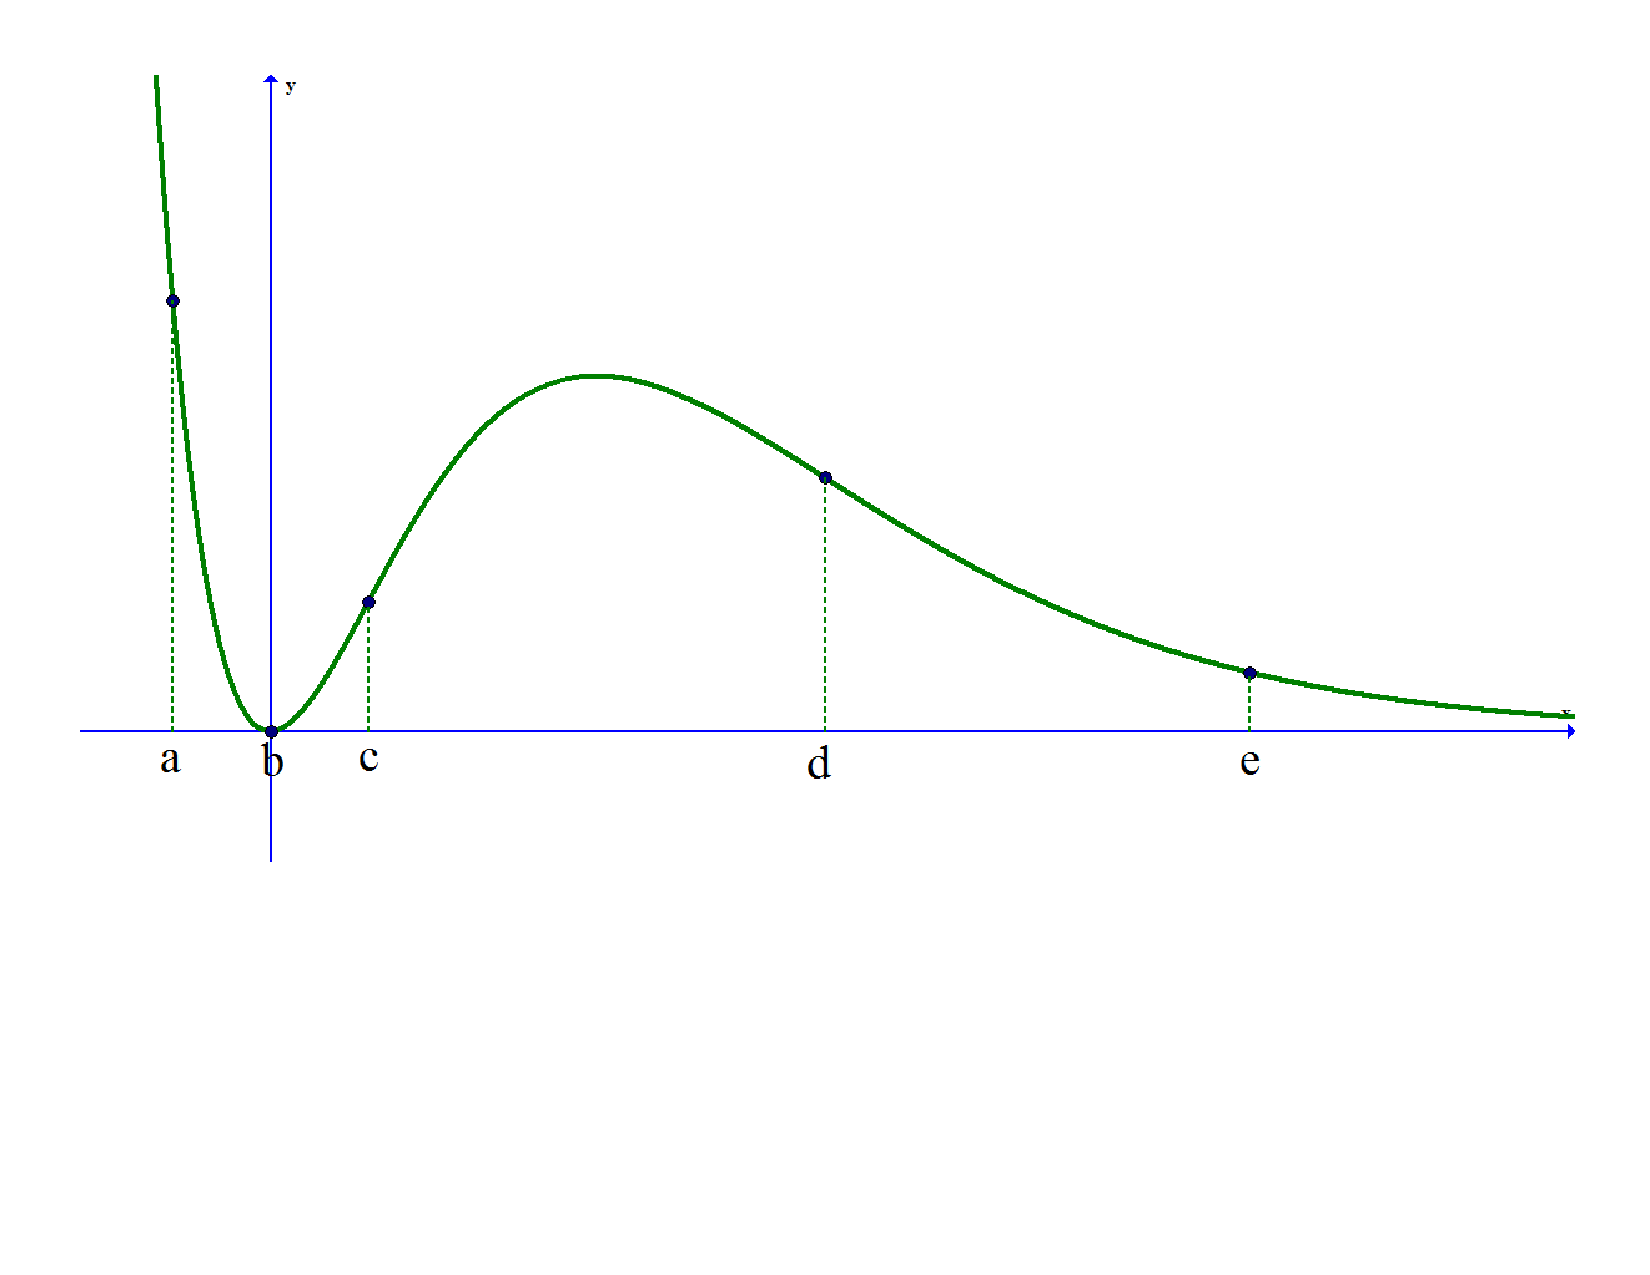
\includegraphics[scale=0.45]{graph.pdf}
\end{center}

Arrange $f^{\prime}(a)$, $f^{\prime}(b)$, $f^{\prime}(c)$, $f^{\prime}(d)$, and $f^{\prime}(e)$ in increasing order.

\ifans{\fbox{$f^{\prime}(a)<f^{\prime}(d)<f^{\prime}(e)<f^{\prime}(b)<f^{\prime}(c)$}} \fi

\item For each of the following, sketch the graph of the given function and determine where the function is not differentiable. Explain.

\begin{enumerate}

\item $f(x) = |x+2|$ 

\ifans{\fbox{\parbox{1\linewidth}{\begin{center}
$f(x)$ is not differentiable when $x=-2$.\\
The graph has a "sharp corner" at this point.\\
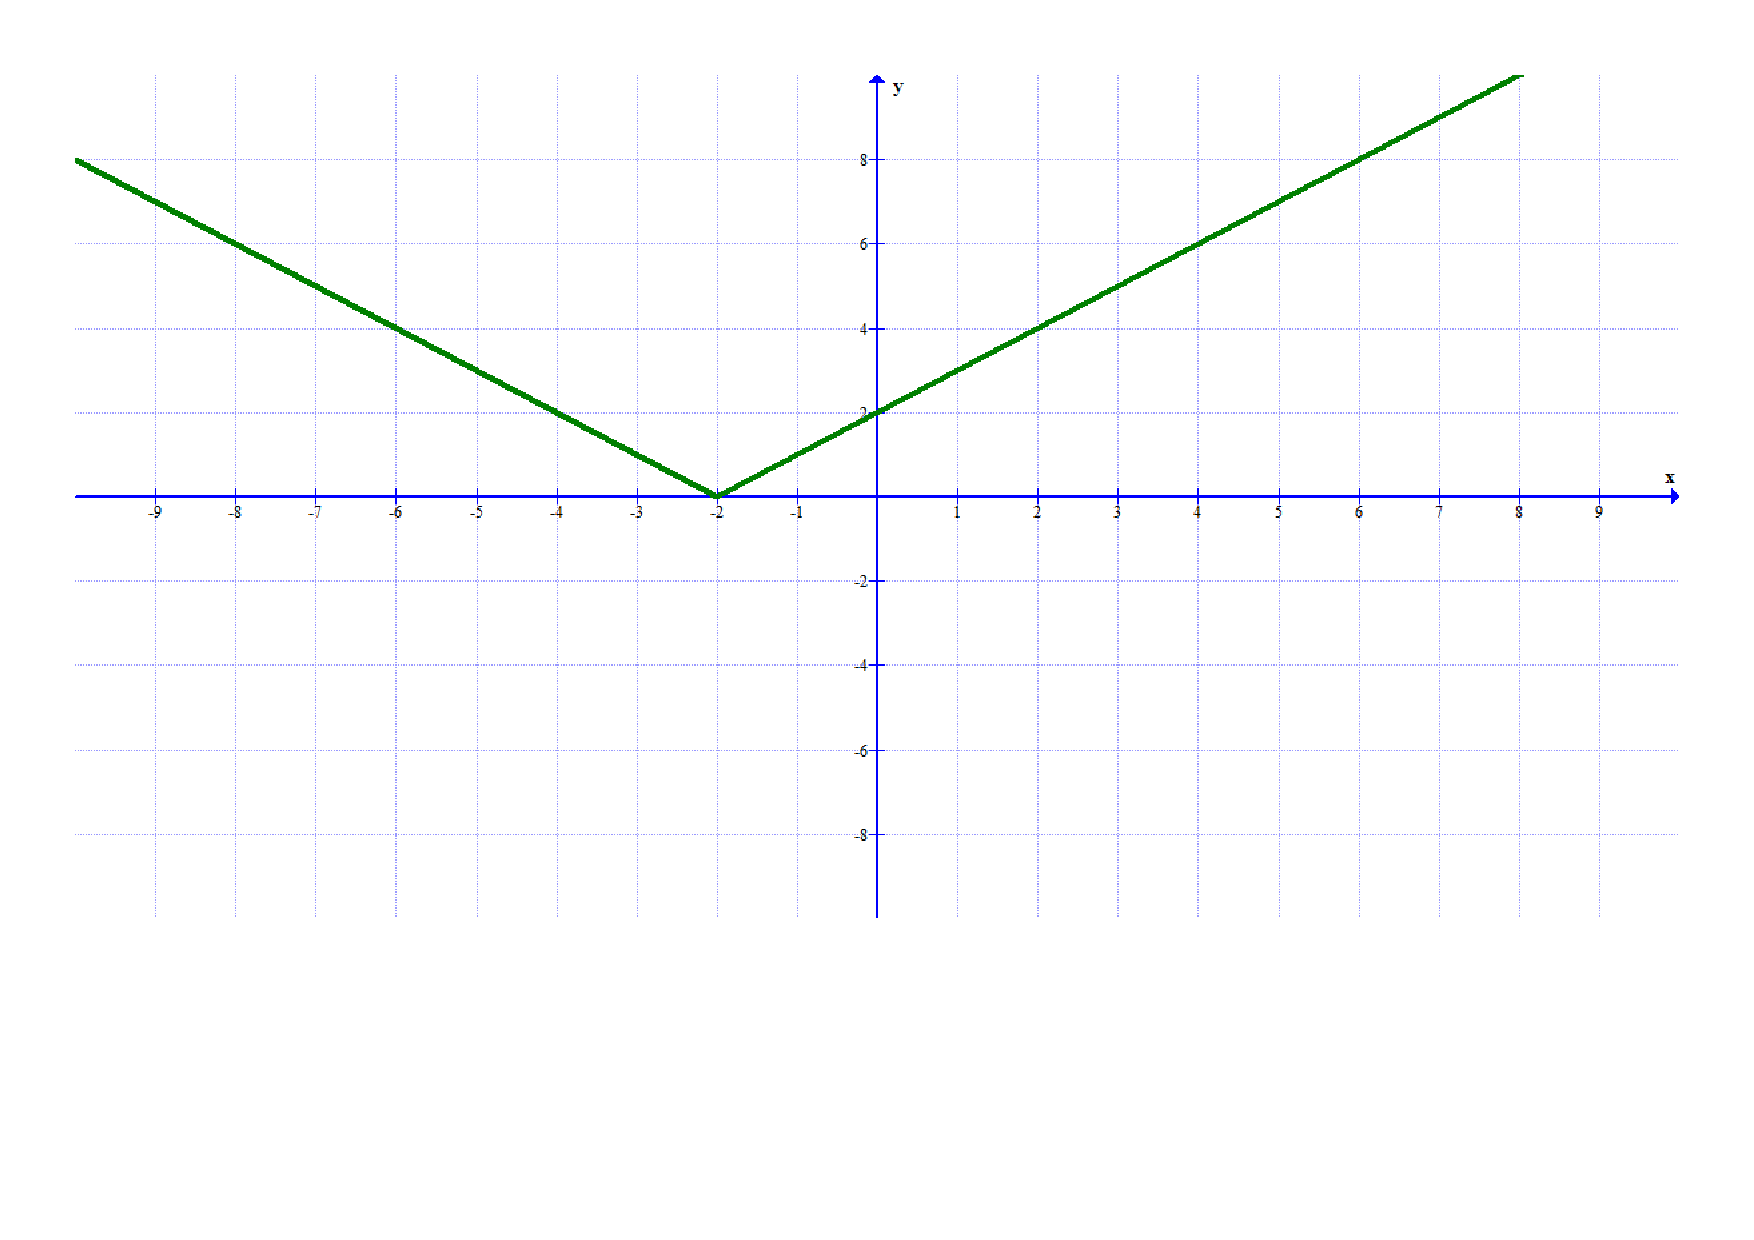
\includegraphics[scale=0.4]{ndiff1.pdf}
\end{center}}}} \fi

\item $\displaystyle f(x) = \sqrt[3]{x}$ 

\ifans{\fbox{\parbox{1\linewidth}{\begin{center}
$f(x)$ is not differentiable at $x=0$.\\
It has a vertical tangent line at this point.\\
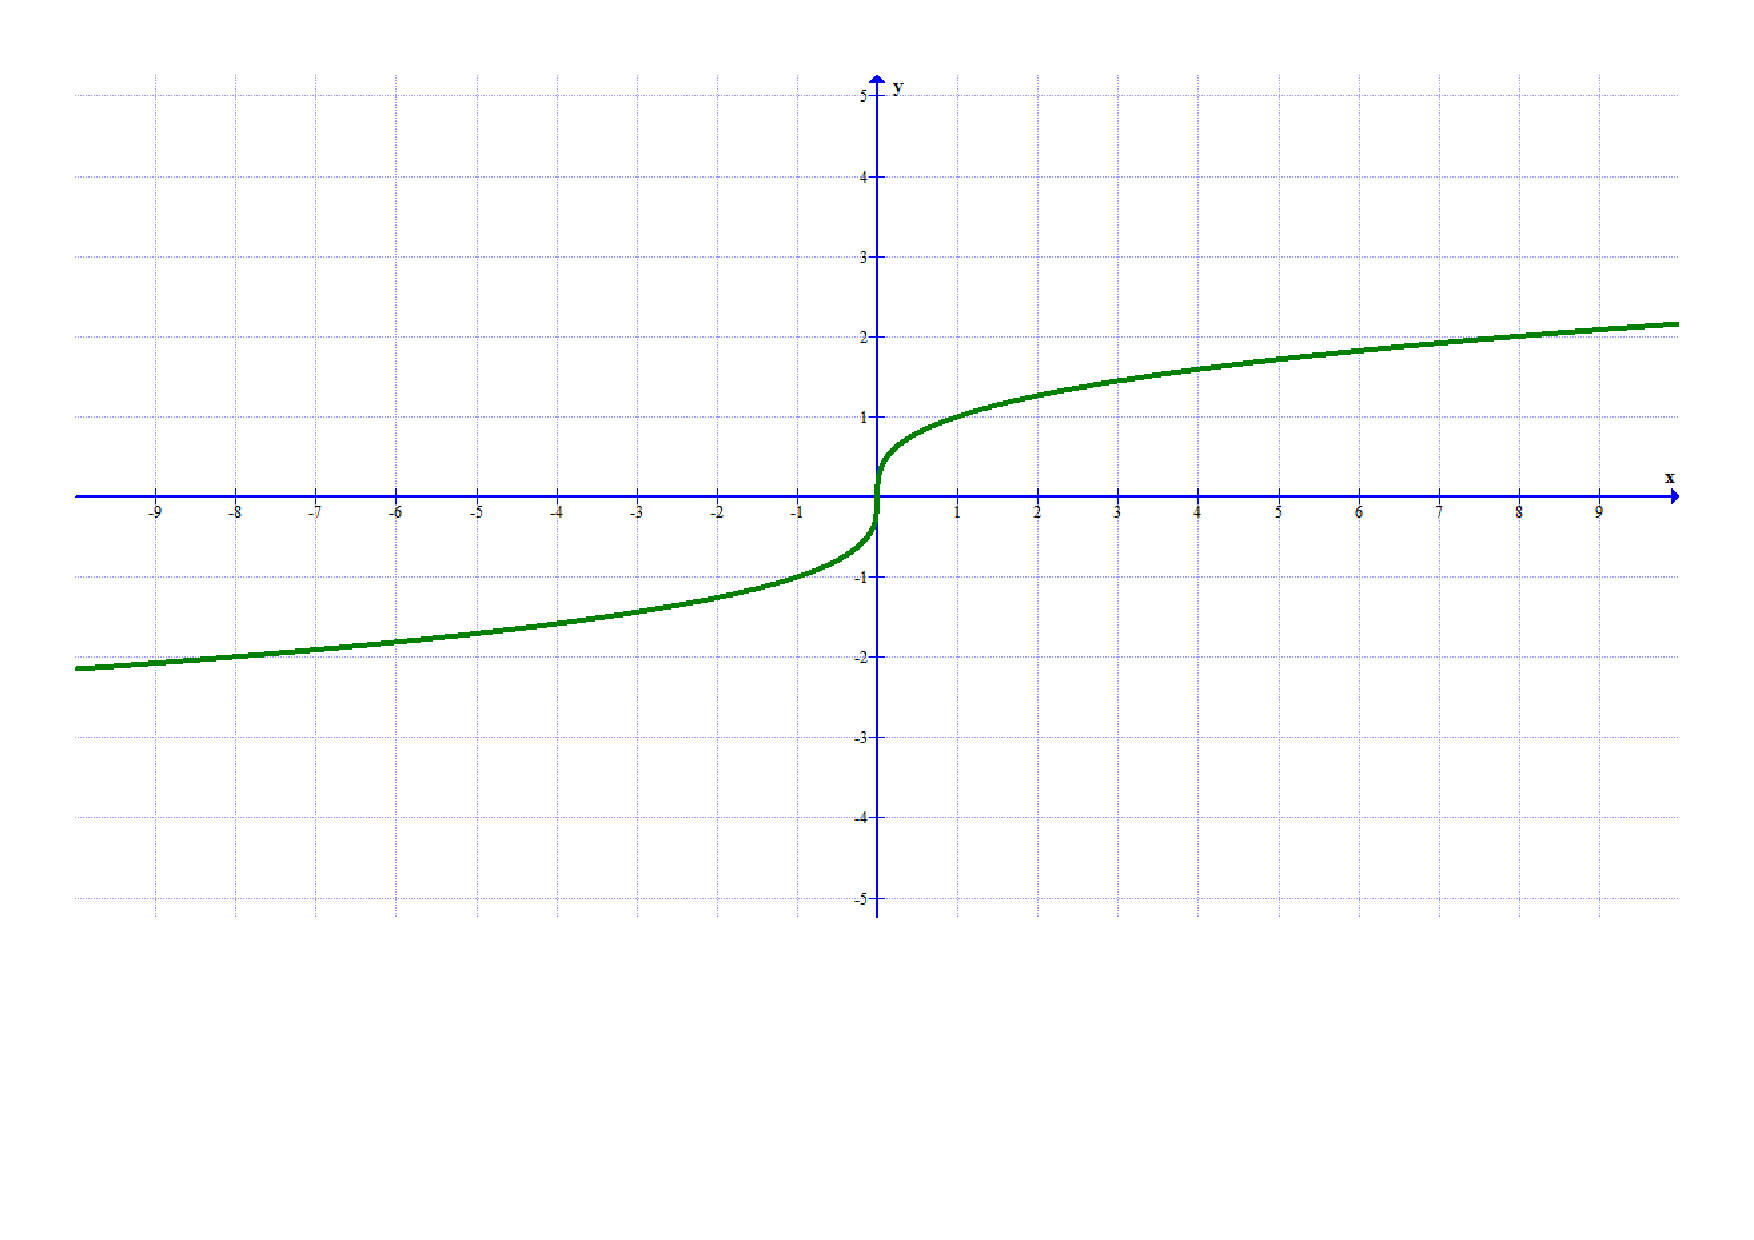
\includegraphics[scale=0.4]{ndiff2.pdf}
\end{center}}}} \fi

\newpage

\item $\displaystyle f(x)=\left\{\begin{array}{lll}
x+1 & \text{if} & x>1\\
x^2 & \text{if} & x \leq 1
\end{array}\right.$

\ifans{\fbox{\parbox{1\linewidth}{\begin{center}
$f(x)$ is not differentiable at $x=1$.\\
The graph is not continuous at this point.\\
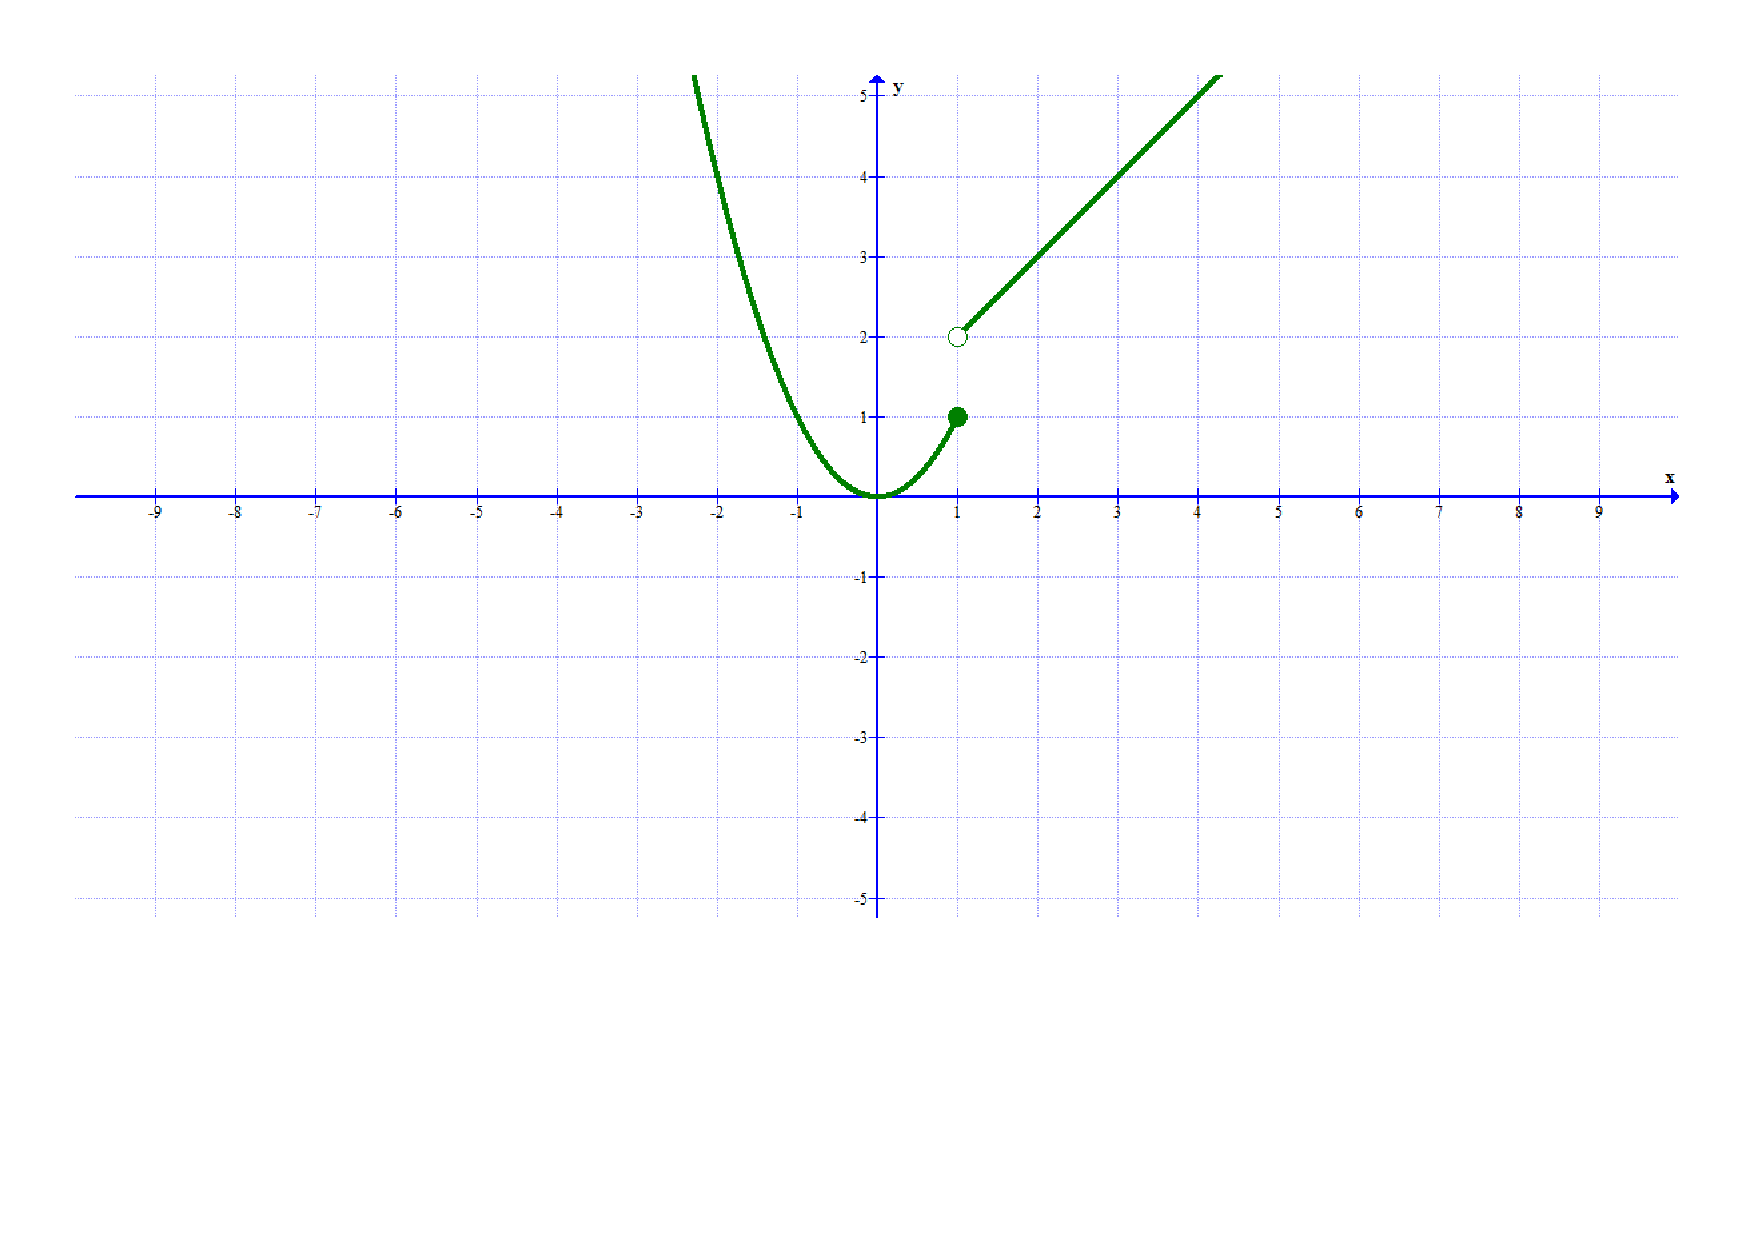
\includegraphics[scale=0.4]{ndiff3.pdf}
\end{center}}}} \fi

\end{enumerate}

\item {\bf Multiple Choice:} If the function $y=f(x)$ is not differentiable at $x=0$, then which of the following MUST be true?

\begin{enumerate}

\item $f(0)$ is undefined.

\item $f(x)$ is NOT continuous when $x=0$.

\item There is a horizontal tangent line to the graph of $y=f(x)$ when $x=0$.

\item There is a vertical tangent line to the graph of $y=f(x)$ when $x=0$.

\item $\lim_{h\rightarrow 0}\frac{f(0+h)-f(0)}{h}$ does not exist.

\end{enumerate}

\newpage

\item Match each of the graphs for functions (a)-(d) with the appropriate graph of its derivative (i)-(iv).\\

\begin{center}
\begin{tabular}{cc|cc}
(a) && (i)&\\
&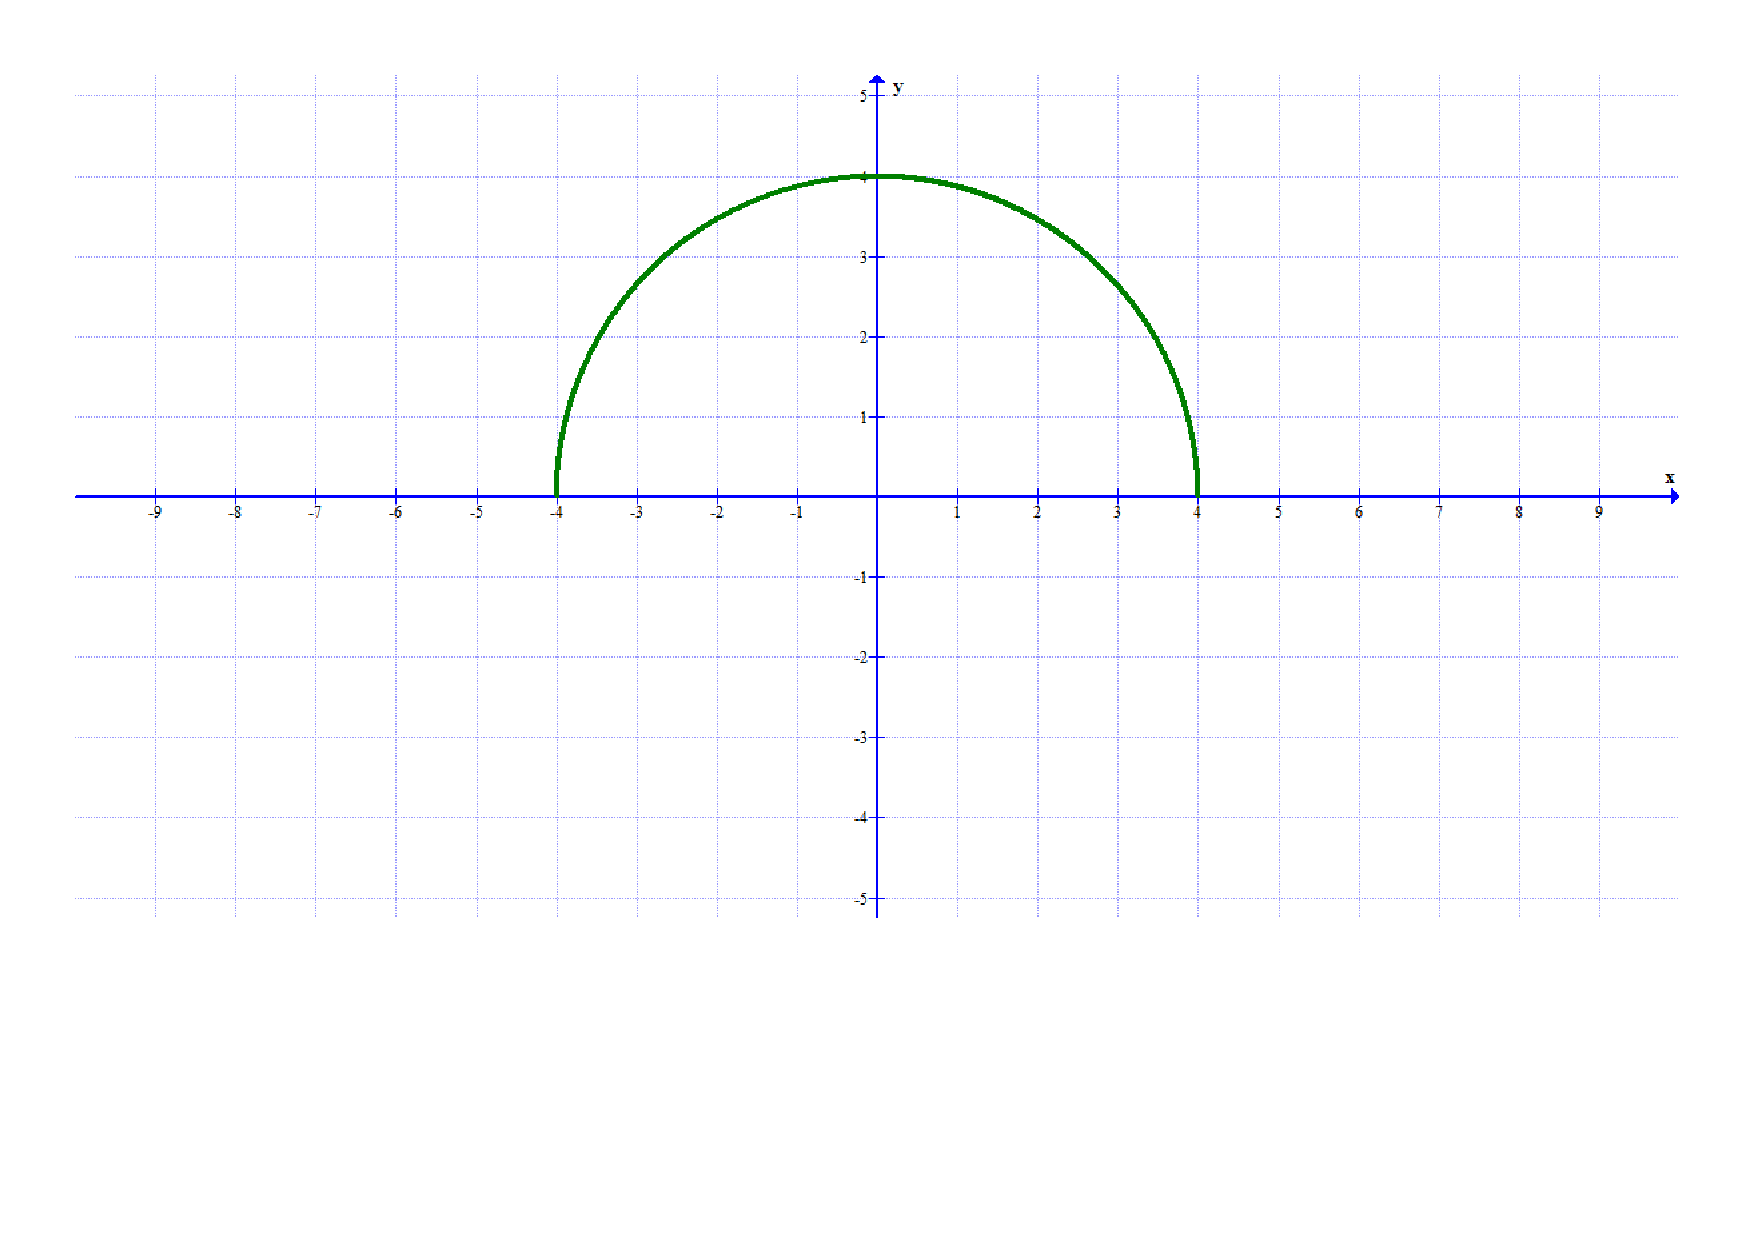
\includegraphics[scale=0.22]{match1.pdf}& & 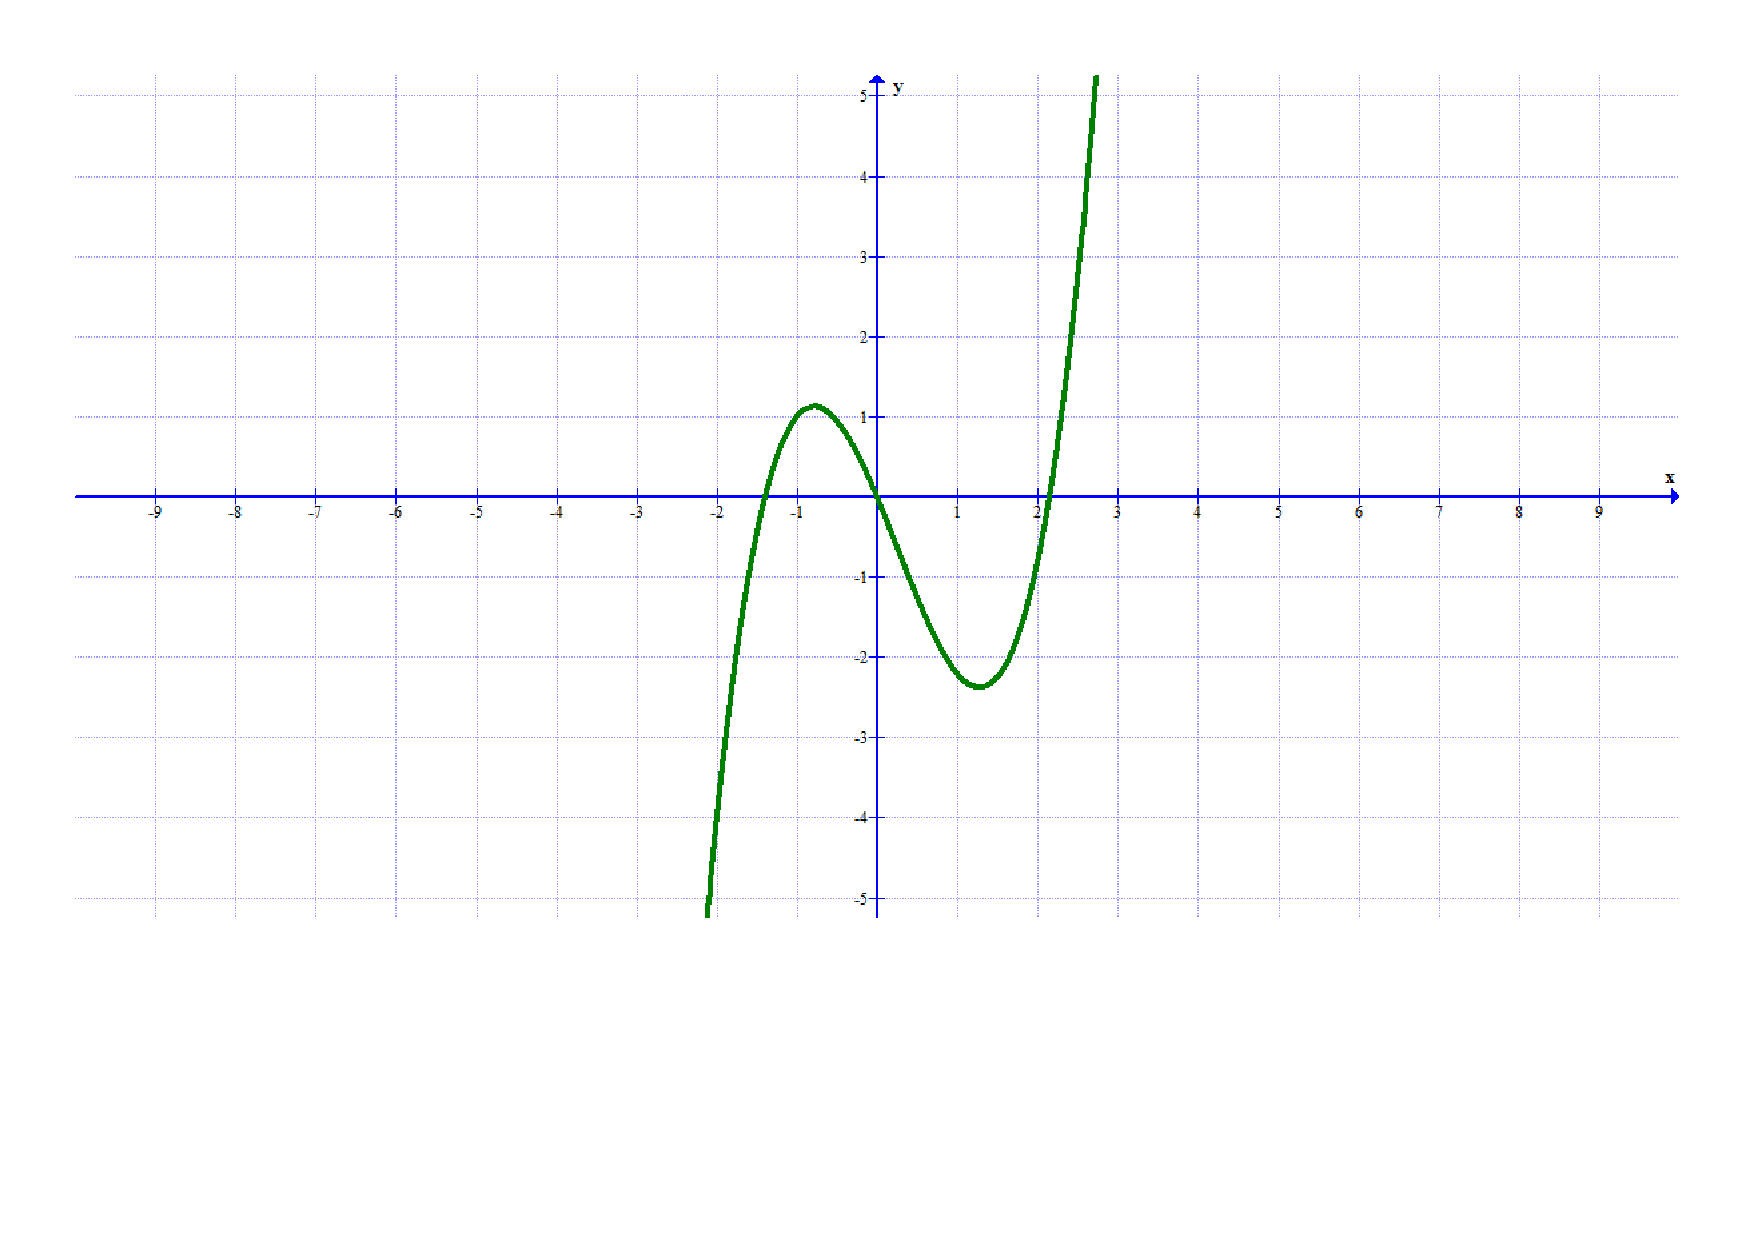
\includegraphics[scale=0.22]{matchd.pdf}\\
(b) && (ii)&\\
&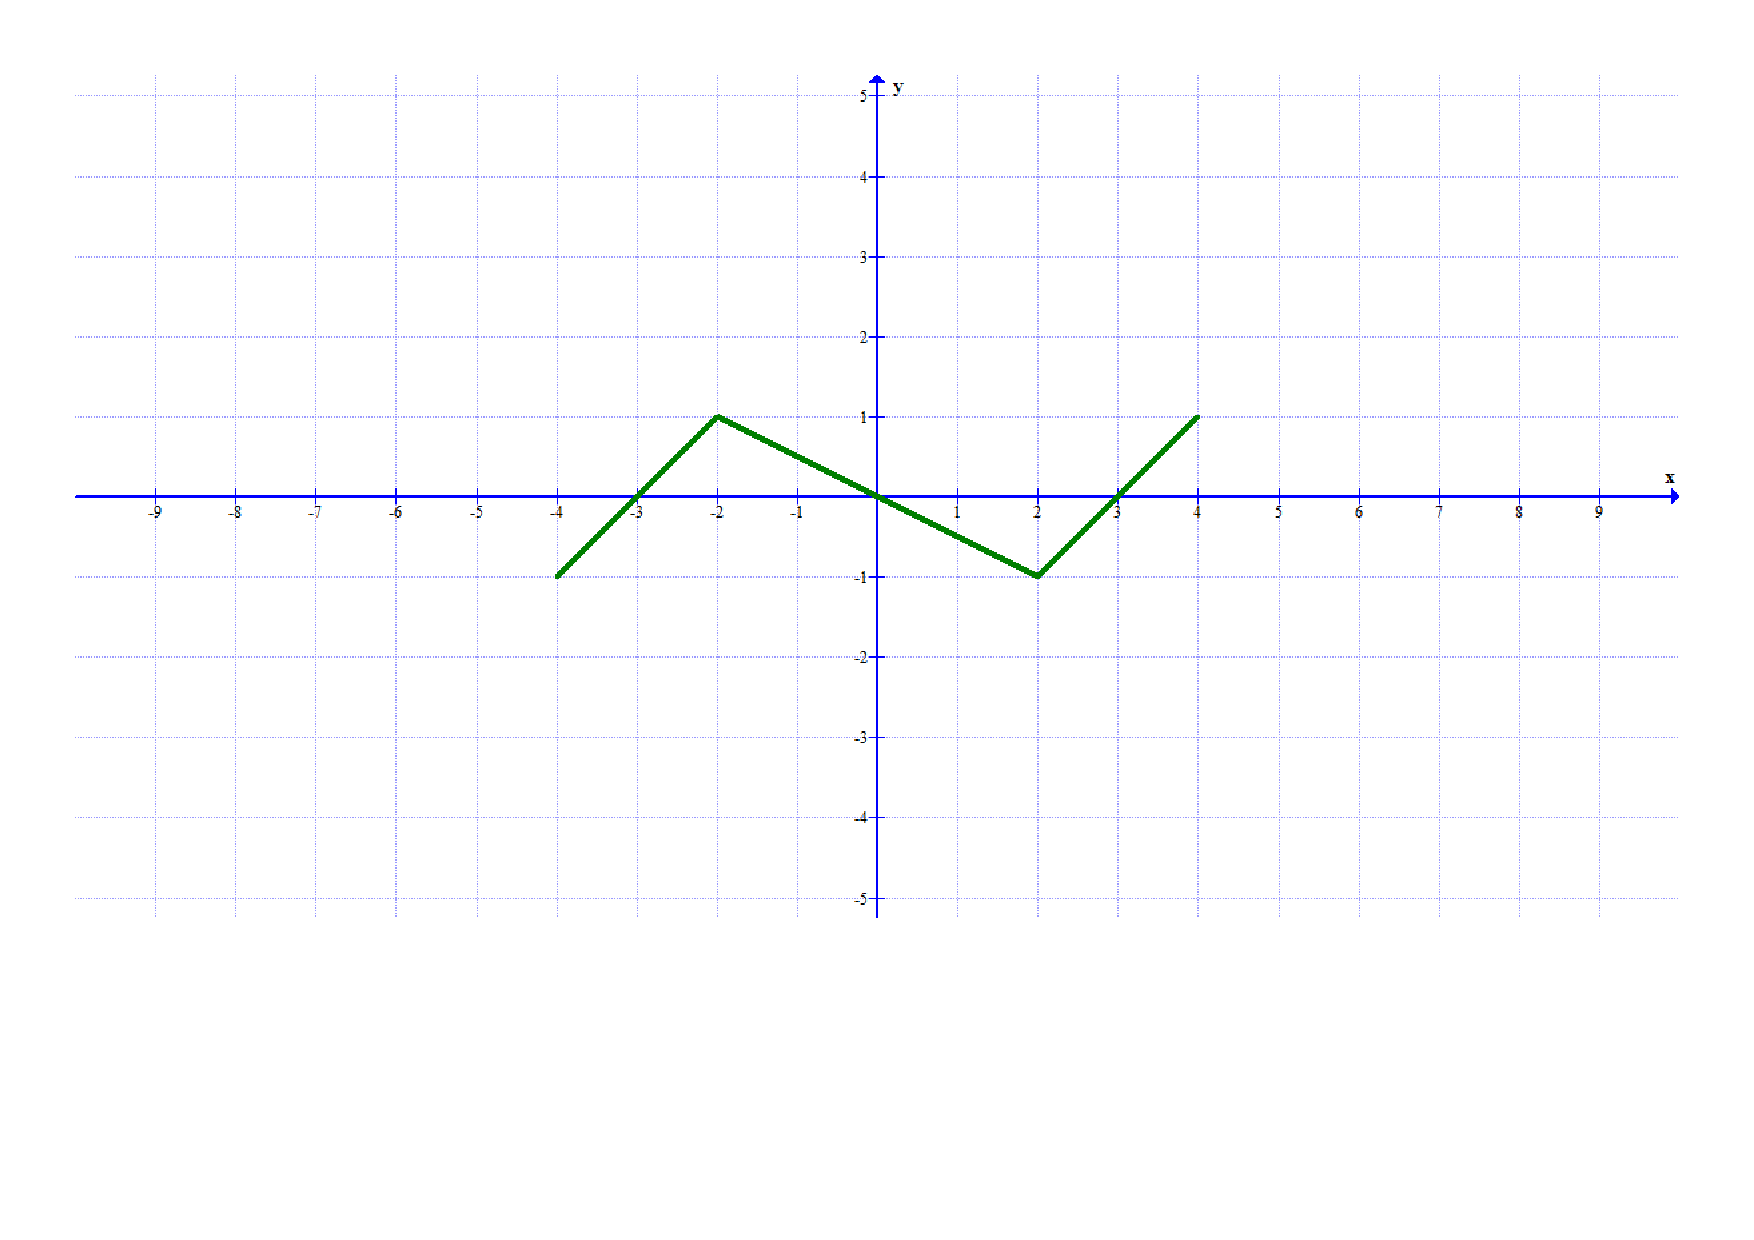
\includegraphics[scale=0.22]{match2.pdf} & &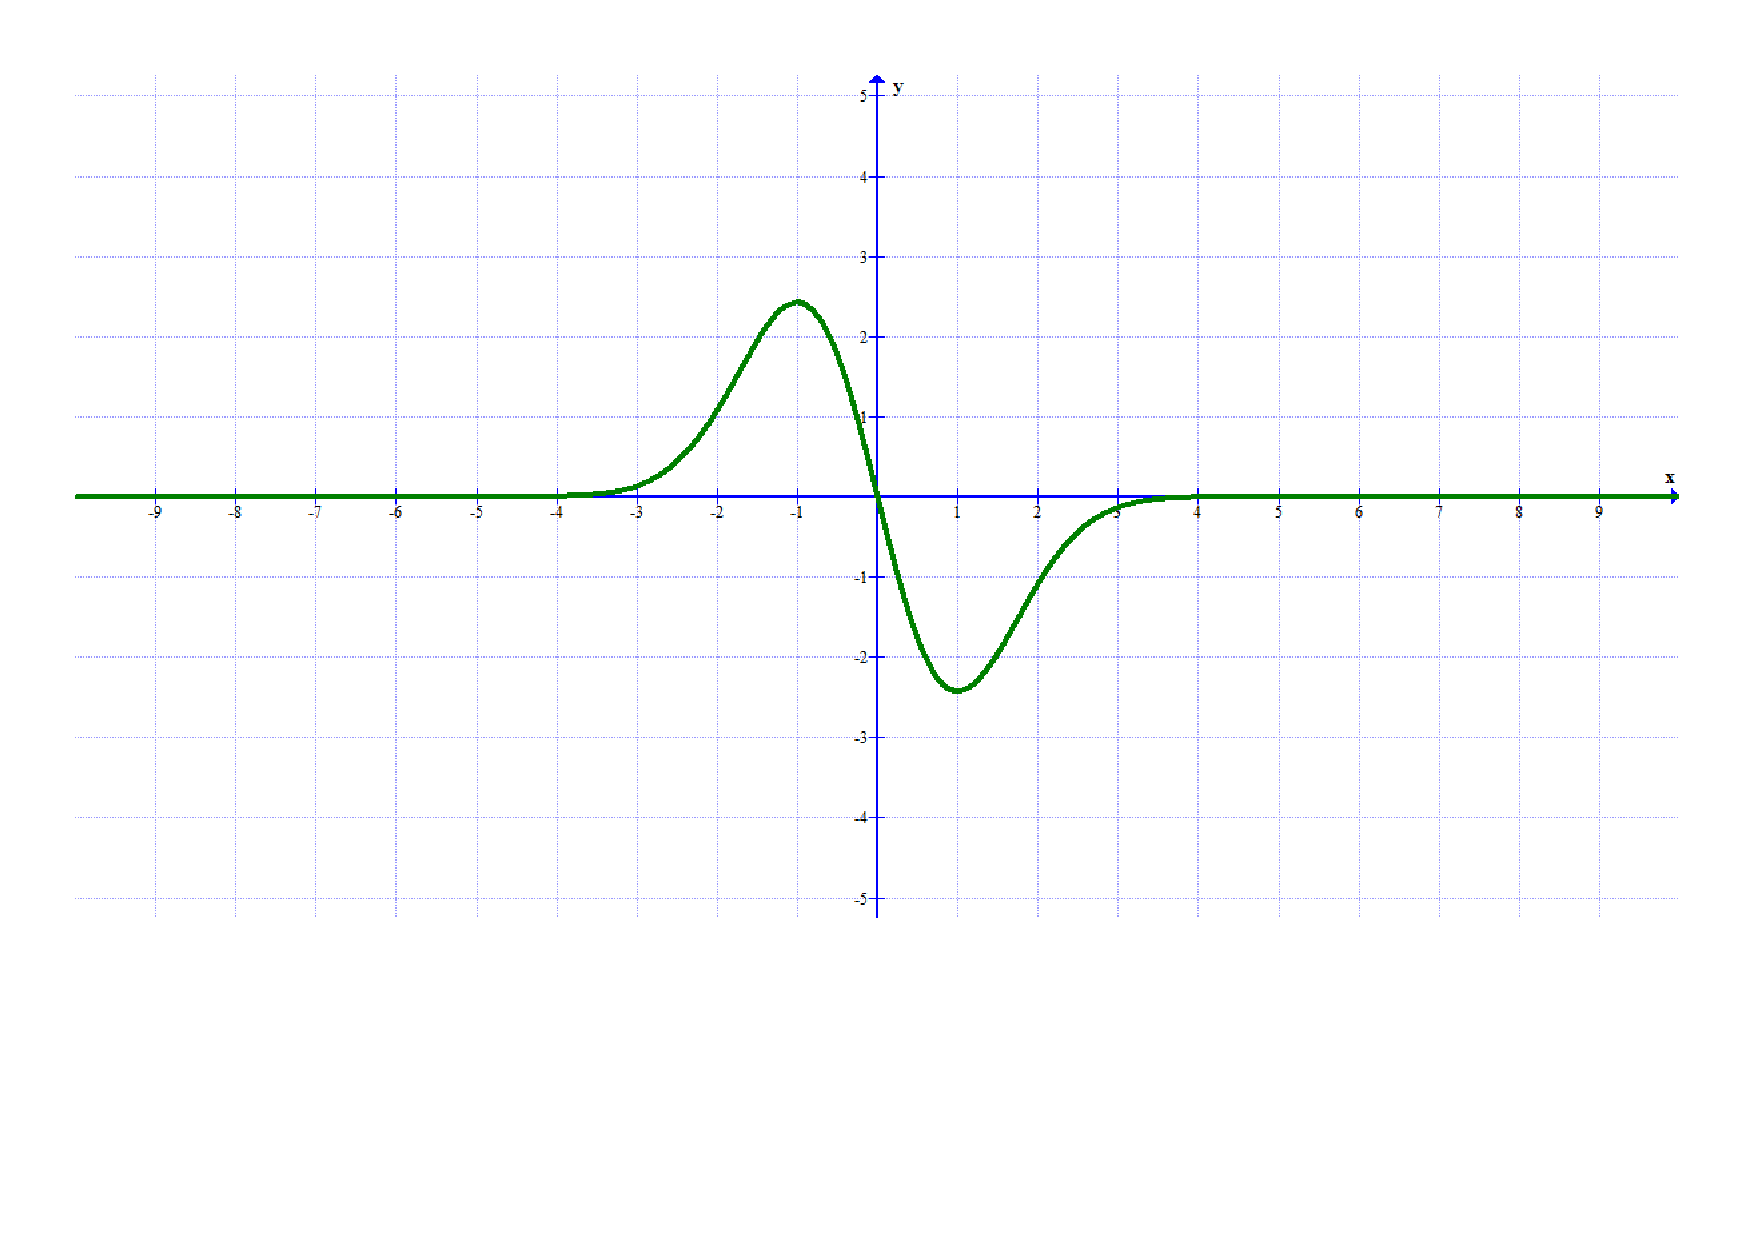
\includegraphics[scale=0.22]{matchc.pdf}\\
(c) && (iii)&\\
&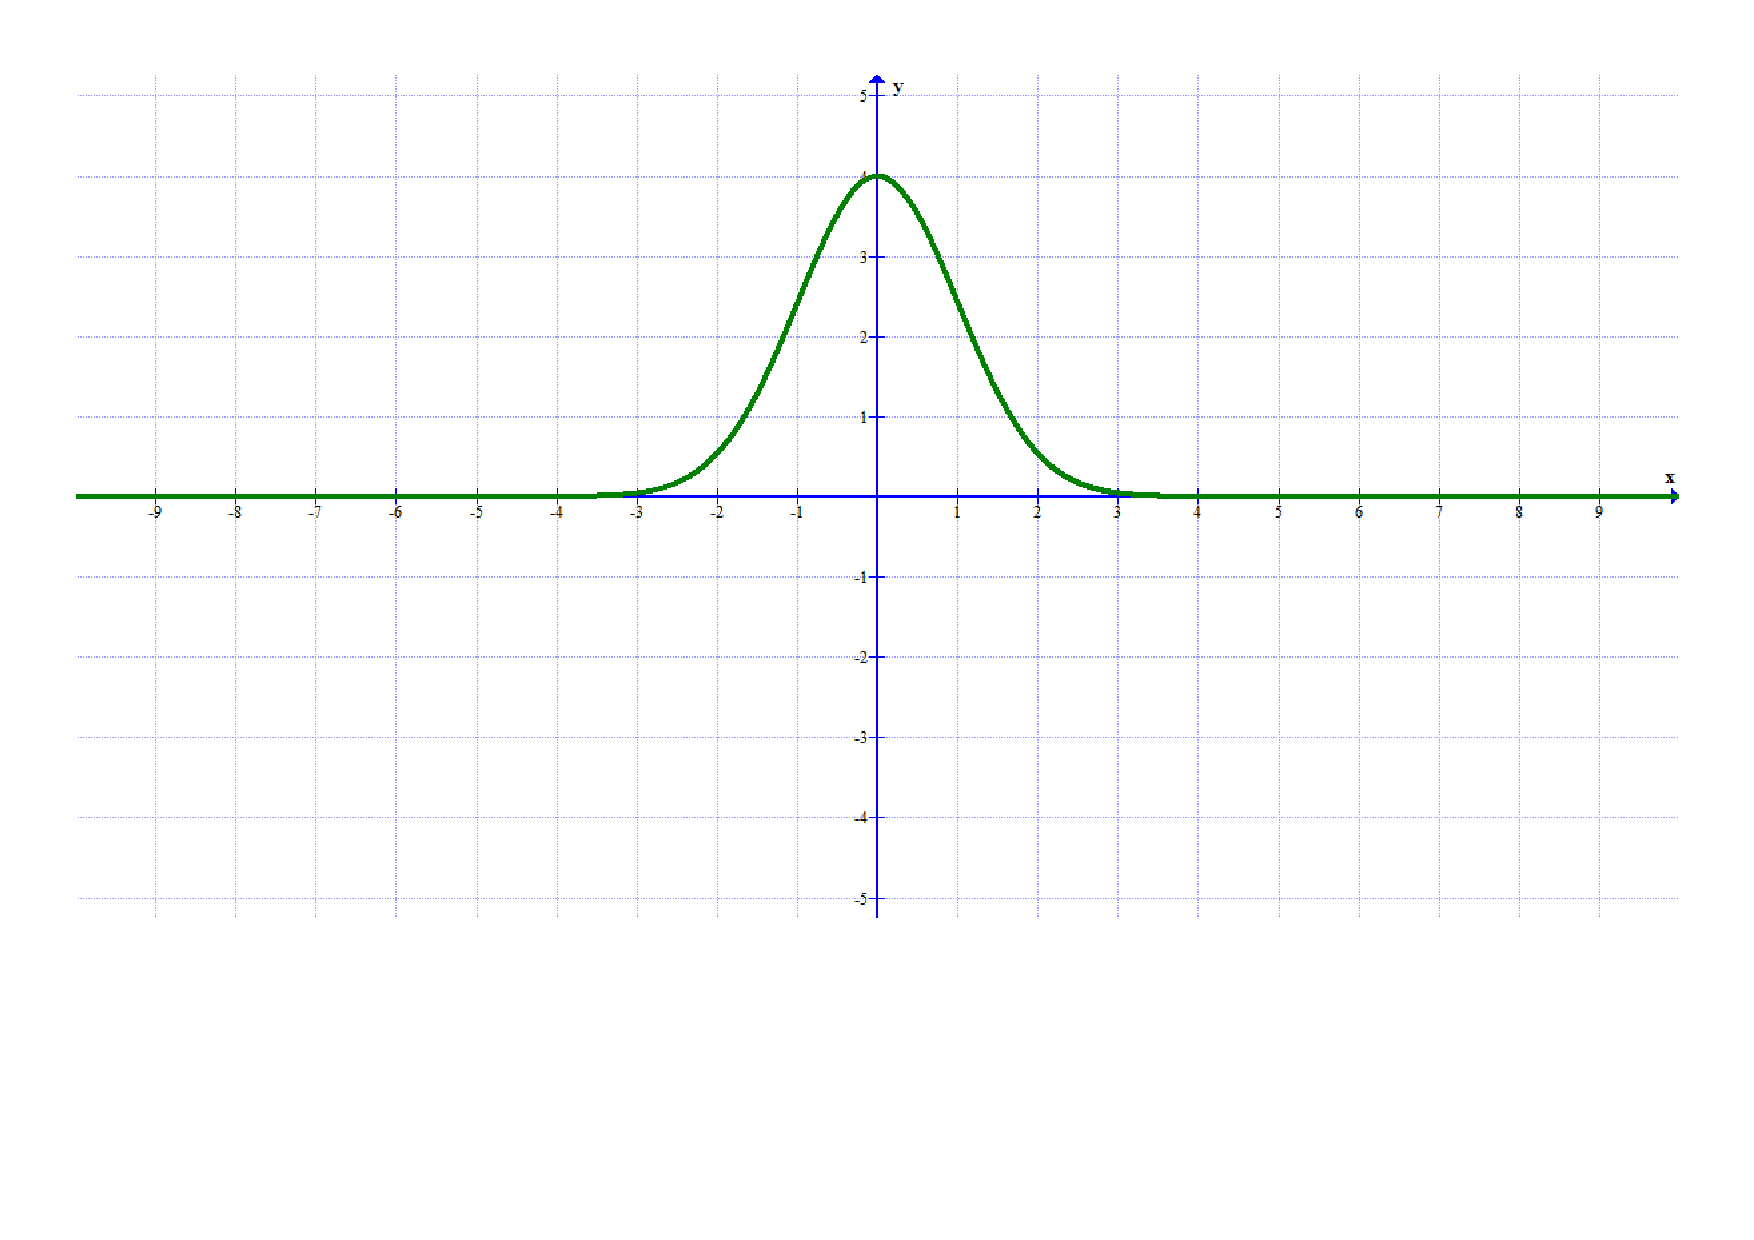
\includegraphics[scale=0.22]{match3.pdf} & & 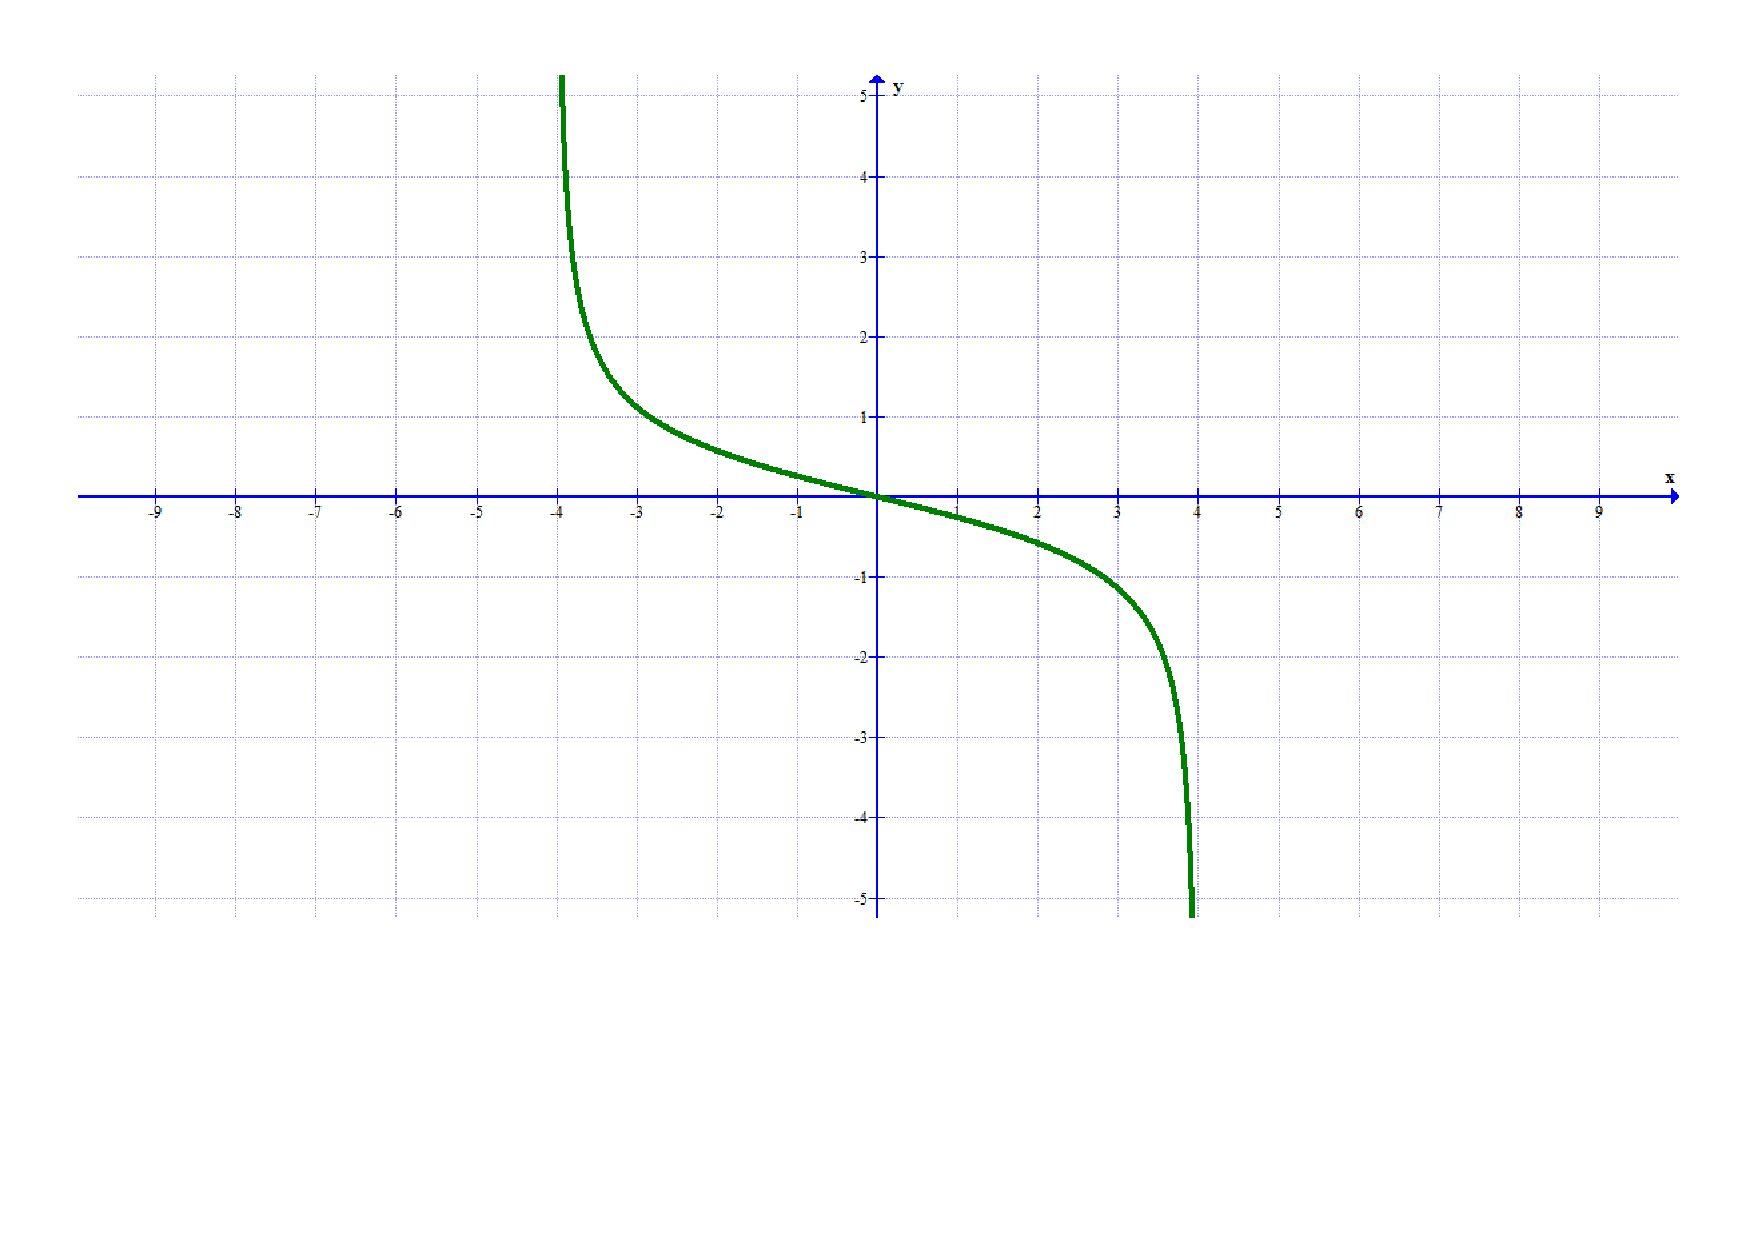
\includegraphics[scale=0.22]{matcha.pdf}\\
(d) && (iv)&\\
&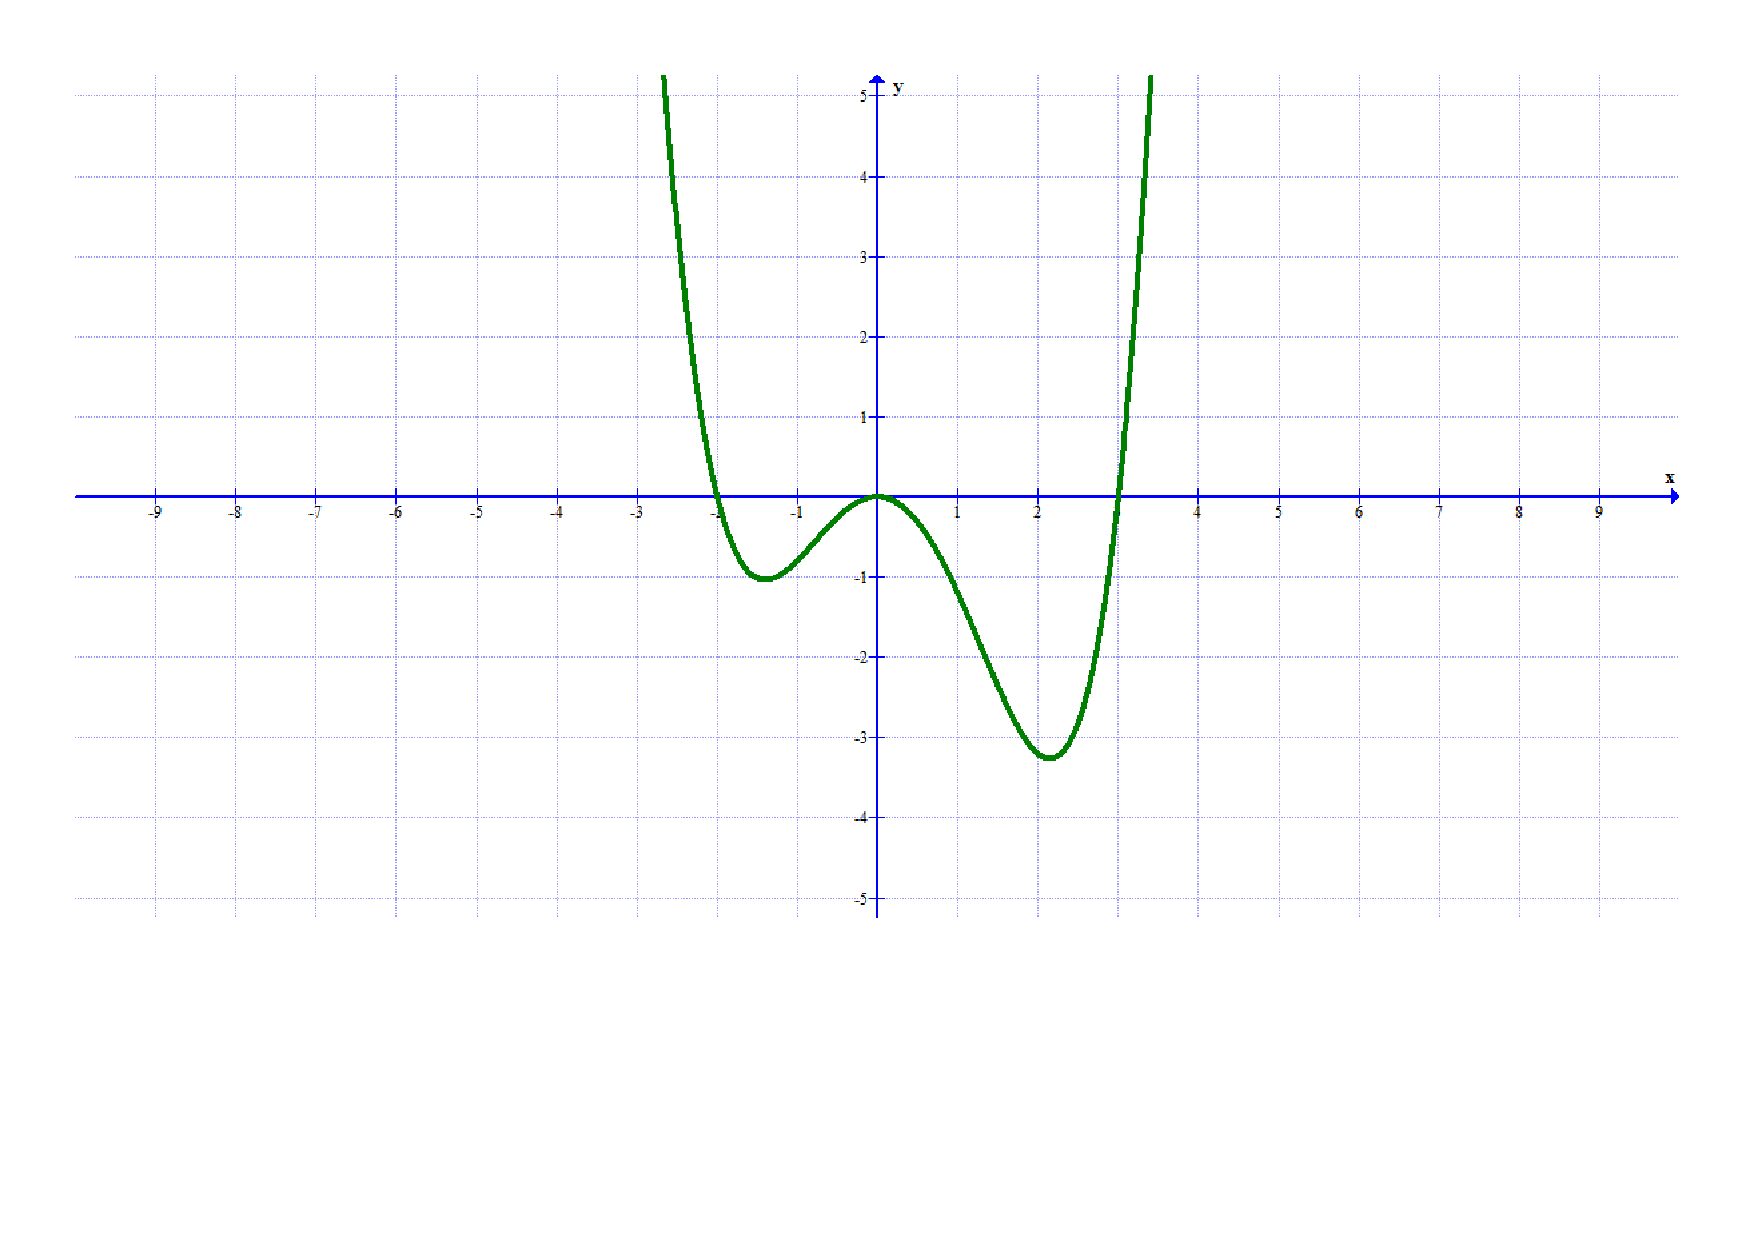
\includegraphics[scale=0.22]{match4.pdf} & & 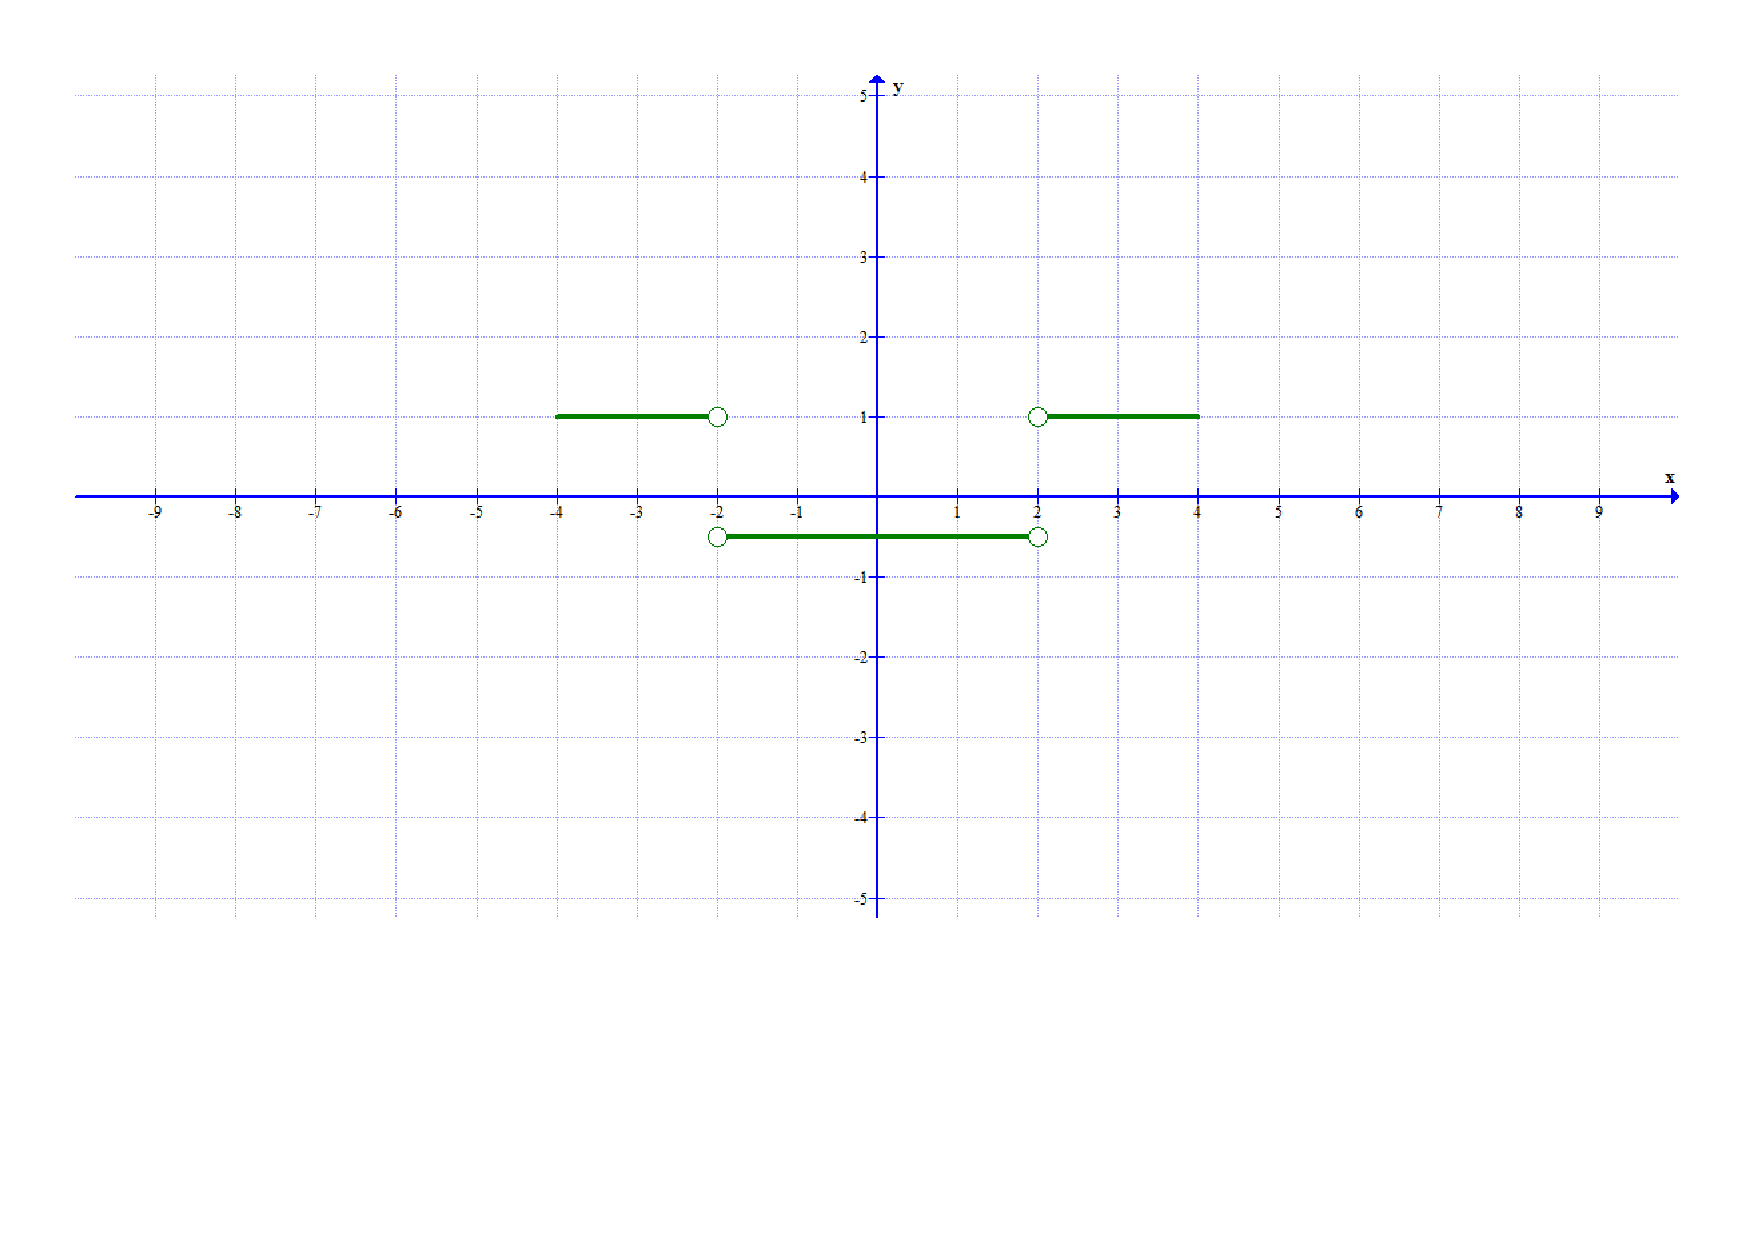
\includegraphics[scale=0.22]{matchb.pdf}
\end{tabular}
\end{center}

\ifans{\fbox{Answer:
\begin{tabular}{|c|c|}
\hline
$f(x)$ & $f^{\prime}(x)$\\
\hline
(a) & (iii)\\
\hline
(b) & (iv)\\
\hline
(c) & (ii)\\
\hline
(d) & (i)\\
\hline
\end{tabular}}} \fi

\item Sketch a function $y=f(x)$ with the given characteristics. (There are many possible answers.)

\begin{enumerate}

\item $f^{\prime}(x) <0$ when $x<0$; $f^{\prime}(x) >0$ when $x>0$; and $f(0) = 0$.

\ifans{\fbox{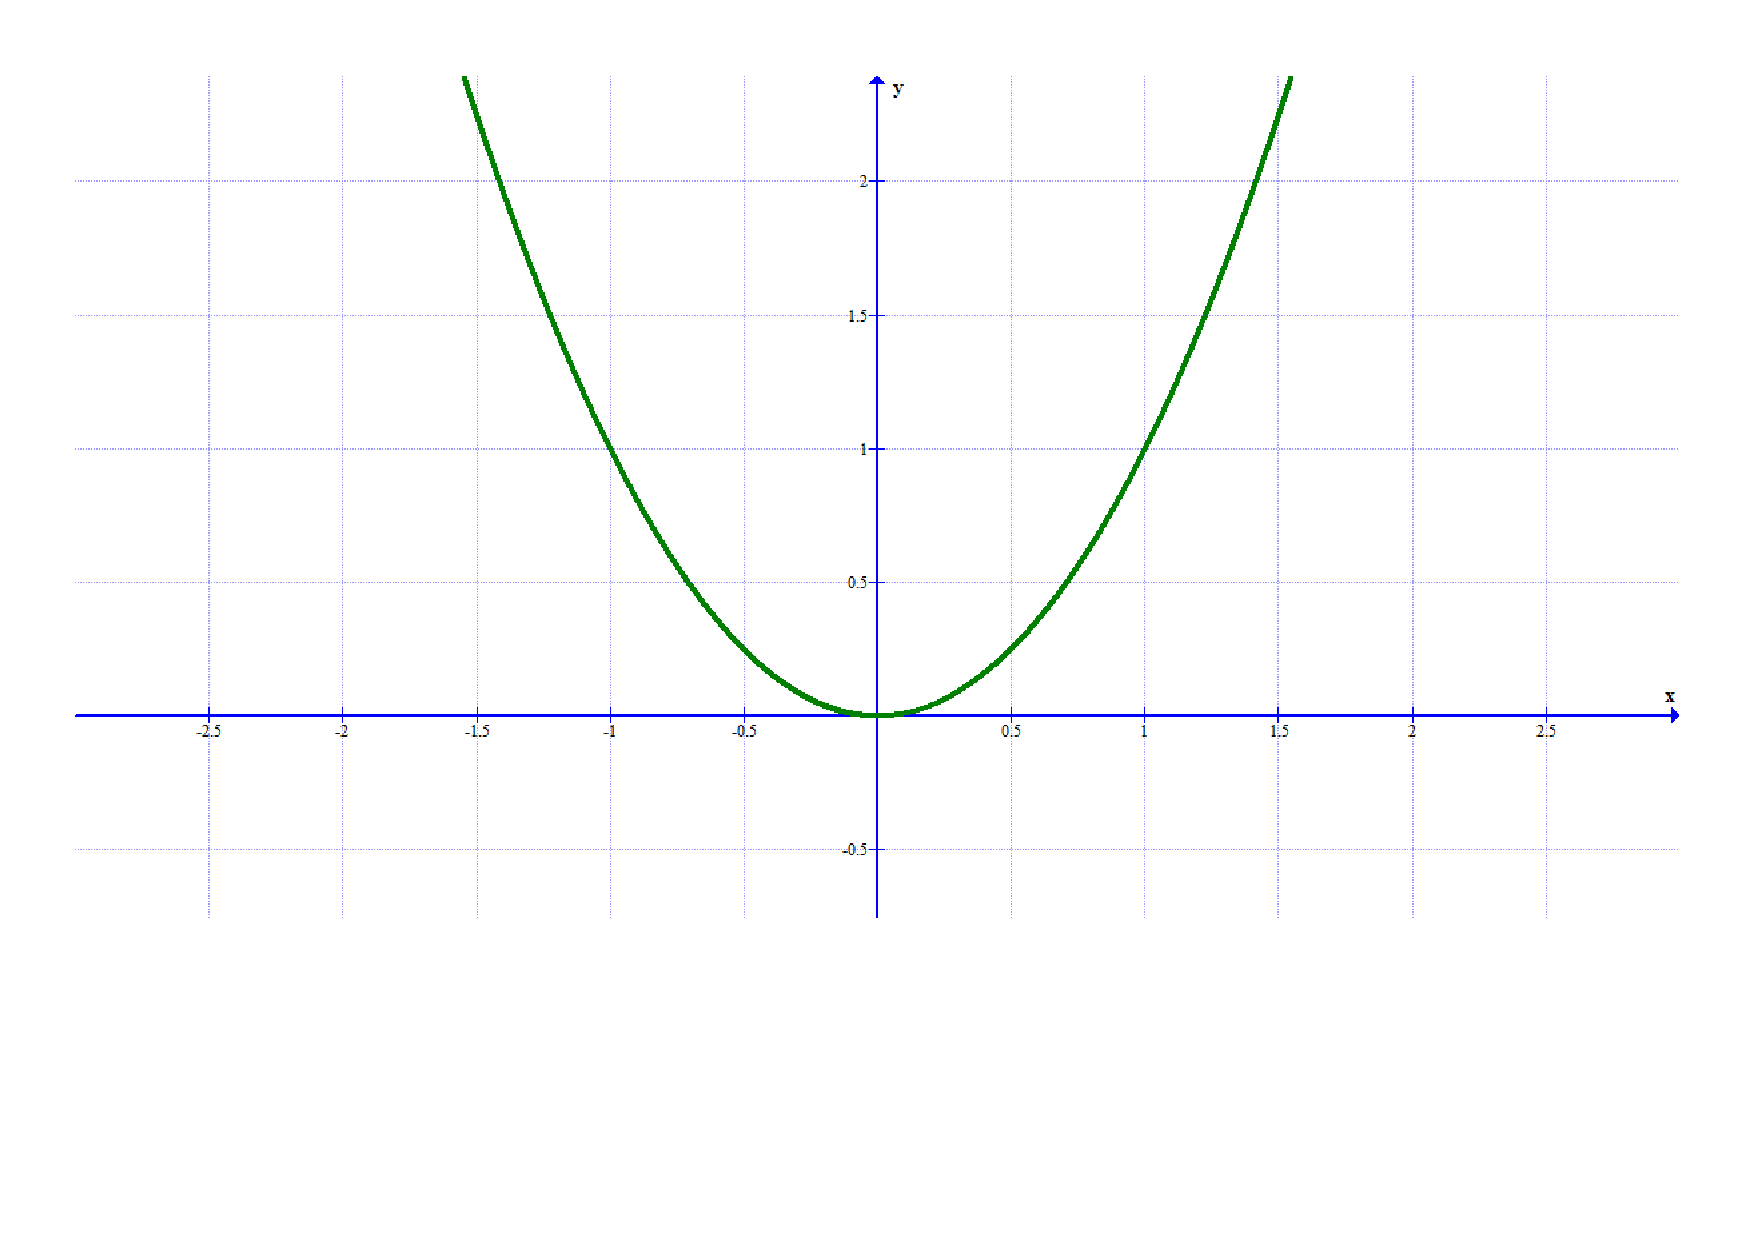
\includegraphics[scale=0.35]{graph1.pdf}}} \fi

\item $f^{\prime}(x) = 0$ when $x<0$; $f^{\prime}(x) <0$ when $x>0$; and $f(-1) = 3$; $f^{\prime}(0)$ DNE.

\ifans{\fbox{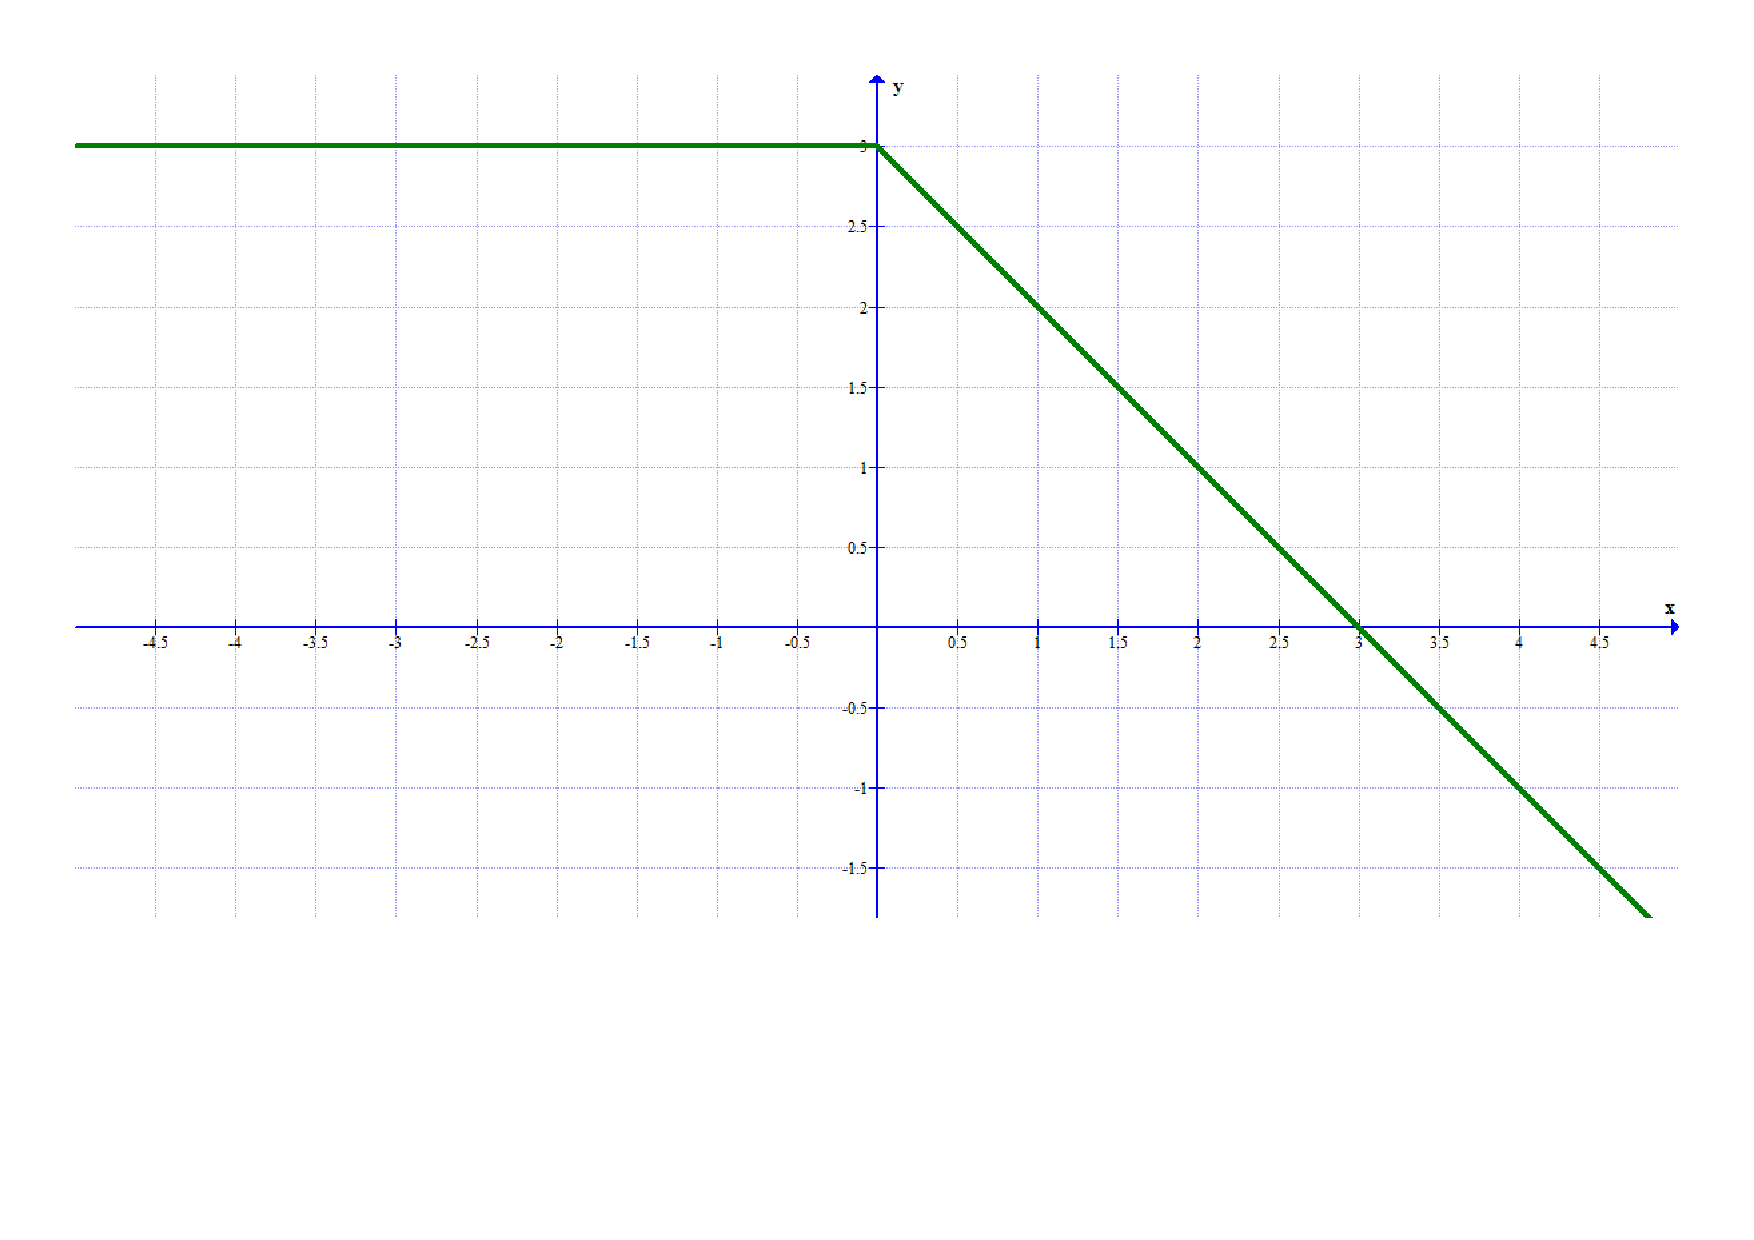
\includegraphics[scale=0.35]{graph2.pdf}}} \fi

\item $f^{\prime}(x) >0$ when $x<-1$ and when $x>1$; $f^{\prime}(x) < 0$ when $-1<x<1$.  

\ifans{\fbox{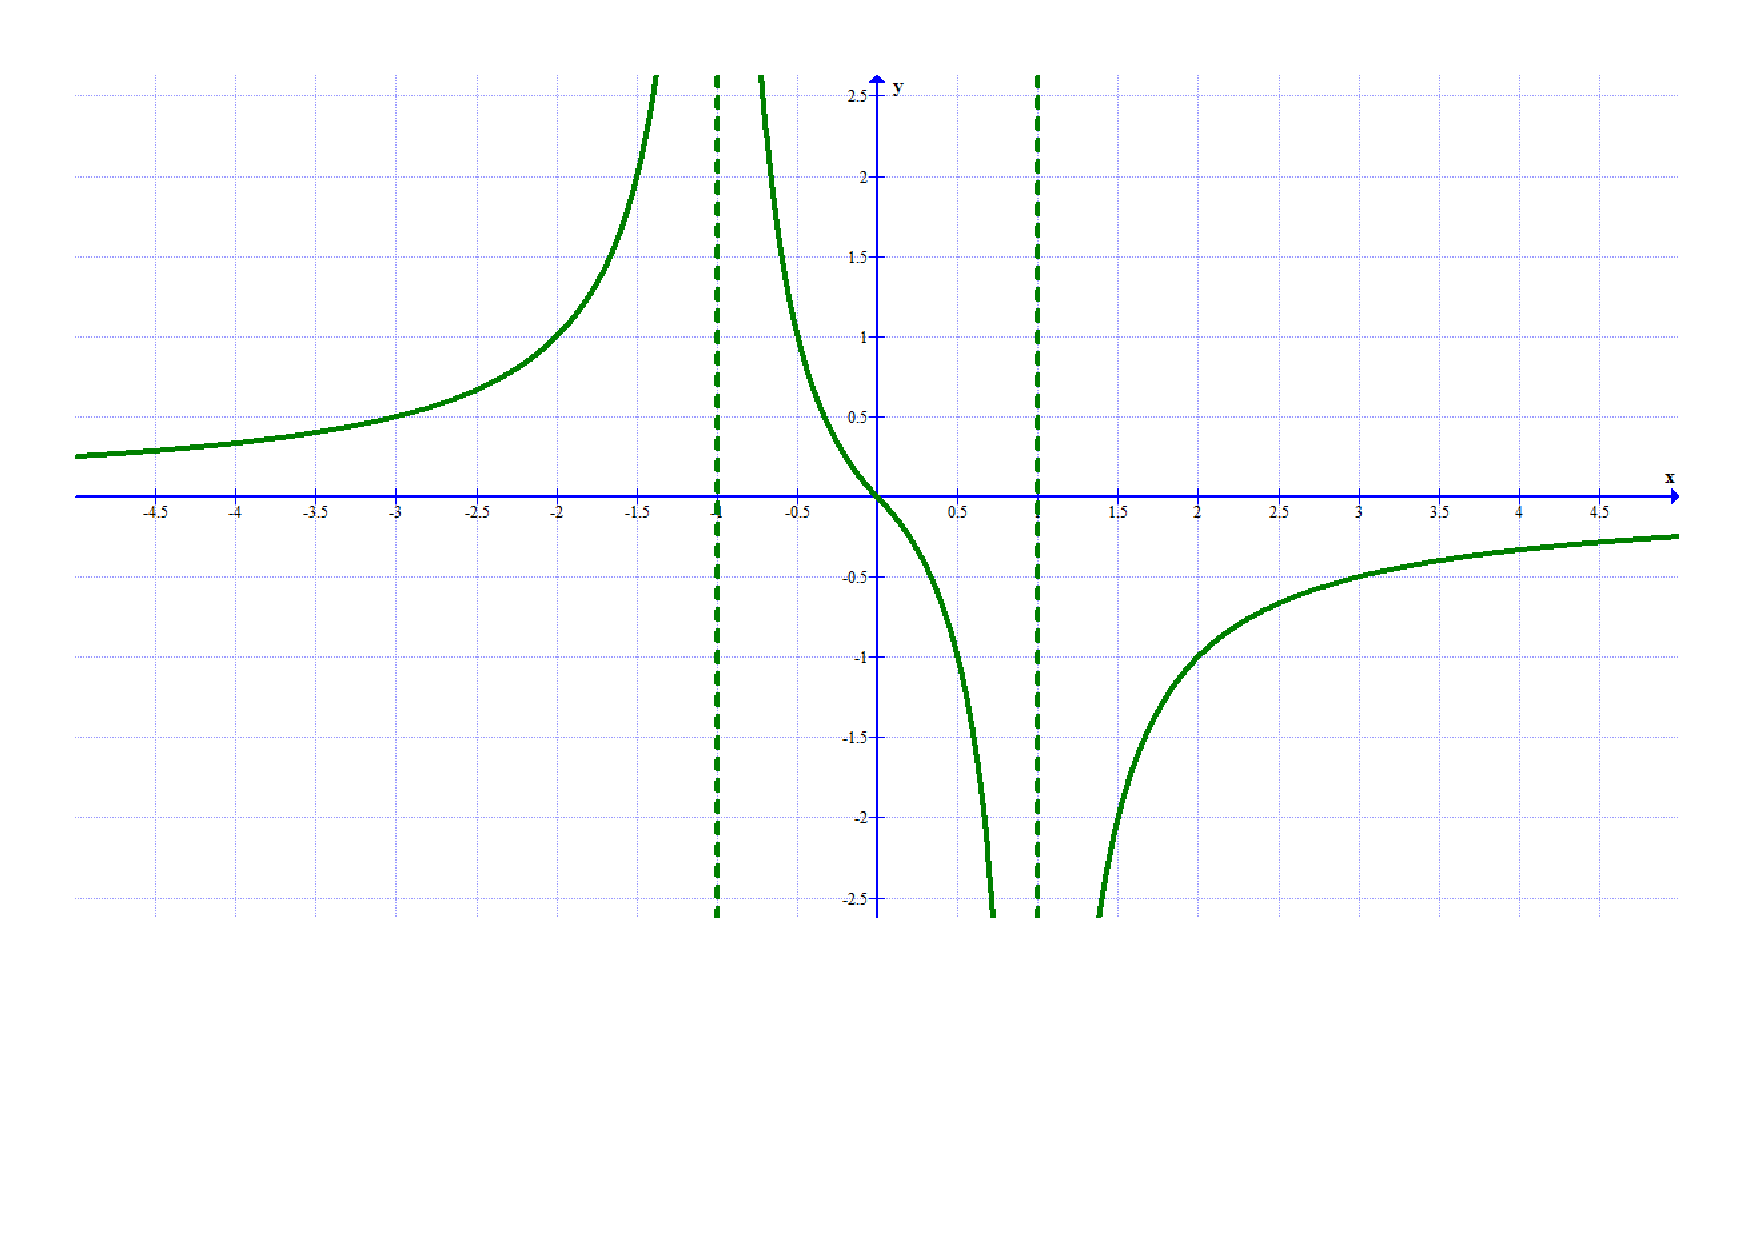
\includegraphics[scale=0.35]{graph3.pdf}}} \fi

\newpage

\item $f(x)$ has a vertical tangent line when $x=1$; $f^{\prime}(x)>0$ for $x < 1$; $f(x)$ is not differentiable when $x=-1$.

\ifans{\fbox{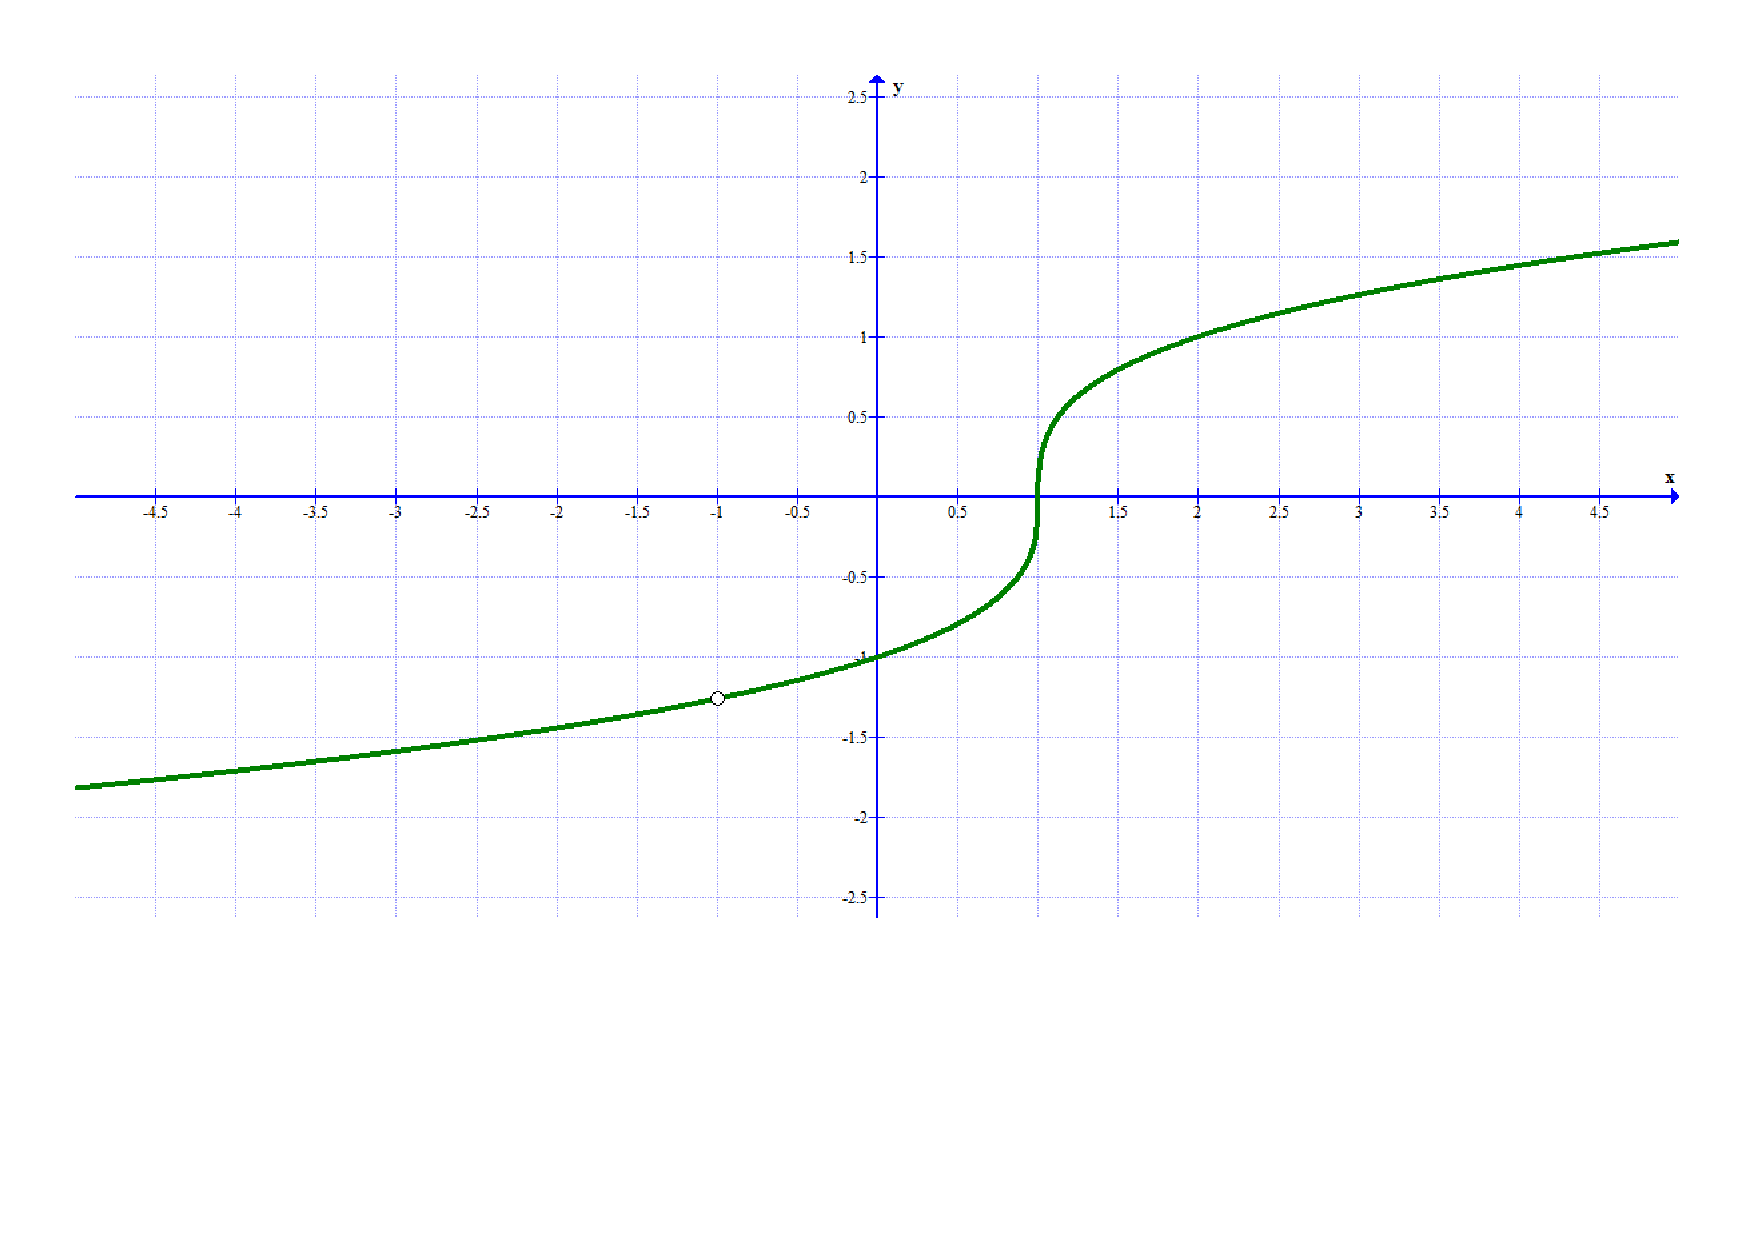
\includegraphics[scale=0.35]{graph4.pdf}}} \fi

\end{enumerate}

\end{enumerate}

\end{document}